\documentclass{article}
\usepackage[utf8]{inputenc}
\usepackage{geometry}
\usepackage{longtable}
\usepackage{graphicx} % For including images
\usepackage{hyperref} % For hyperlinks
\usepackage{enumitem}
\usepackage{graphicx}
\usepackage{booktabs} % For professional looking tables
\usepackage{float} % For improved control over floating environments

\geometry{
 a4paper,
 total={170mm,257mm},
 left=20mm,
 top=20mm,
}

\title{Software Architecture of Train Inter Payment System (TrIP)}
\author{Group 04}
\date{\today}

\begin{document}

\maketitle
\newpage

\tableofcontents
\newpage

\section{Product Introduction}
The Train Inter Payment System (TrIP) is a collaborative project initiated by three railroad tycoons to streamline the payment process for train travel. These tycoons, operating a network connecting towns, industries, and a university, aim to address the interoperability issues of their existing payment systems. TrIP will feature smart payment terminals at each station, enabling direct communication for subscription validation or single-fare payments. This system, underpinned by a service-based architecture, involves critical components like payment terminals and tycoon-specific systems. It's designed with key stakeholder requirements in mind: maintainability and operational efficiency for the owner, usability and reliability for the tycoons, and usability and security for passengers. The project seeks to ensure passengers can easily manage payments and subscriptions across the network, enhancing the overall travel experience while safeguarding user data.
\newpage

\section{Decisions}
\subsection{Decision 1: UI}

\subsection*{Status}
Accepted.

\subsection*{Architectural Summary}
% TODO

\subsection*{Concern}
Passengers require a user interface that is easy to navigate, visually appealing, and provides a seamless experience across different tycoon systems.

\subsection*{Context}
In the context of designing an intuitive and engaging user interface for the TrIP system terminals, we face the challenge of selecting guiding principles and frameworks that will shape the user experience and interaction design.
The design of the user interface on the terminals involves the passenger's interaction with the system, from querying routes to finalizing ticket purchases. It is an essential component of the system that directly affects user satisfaction and system usability.

\subsection*{Criteria}
The decision will be guided by the following criteria:
\begin{itemize}
    \item Consistency in design to provide a unified look and feel across all terminals.
    \item Accessibility to ensure the system is usable by all passengers, including those with disabilities.
    \item Responsiveness so that the interface can adapt to various screen sizes and orientations.
    \item Ease of maintenance and scalability for future enhancements.
    \item Alignment with the latest trends in user interface design and technology.
\end{itemize}

\subsection*{Option 1: Use of Standardized UI Components}
This approach involves adopting a comprehensive design system, such as Google's Material Design or IBM’s Carbon Design System, which offers a robust set of standardized UI components. These components include buttons, forms, toggles, navigation patterns, and more, all designed with consistency and usability in mind. By utilizing these pre-designed components, the development process can be significantly accelerated, as developers and designers will not need to create common UI elements from scratch. This ensures a cohesive look and feel across the entire application, enhancing the user's ability to intuitively navigate the system.
\begin{itemize}
    \item \textbf{Pro:} Significantly reduces development time and ensures UI consistency.
    \item \textbf{Pro:} Both Google's Material Design and IBS's Carbon Design System are open source, hence they would allow developers to easily debug the interface, identify possible bugs, seek for contributions online or even contribute themselves.
    \item \textbf{Con:} May limit unique branding opportunities and design customization. 
    \item \textbf{Con:} Some developers may consider it a limit for their creativity. 
\end{itemize}

\subsection*{Option 2: Custom Designed Interactive Interfaces}
This option focuses on creating bespoke interactive interfaces from the ground up, specifically tailored to the unique needs and brand identity of the TrIP system. This could involve developing custom animations, unique layout designs, and interactive elements that engage users in a novel way. By focusing on custom designs, the TrIP system can distinguish itself from competitors and provide a unique user experience that directly addresses specific user needs and preferences.
\begin{itemize}
    \item \textbf{Pro:} Allows for full creative freedom and the opportunity to innovate.
    \item \textbf{Pro:} Less operational cost, and higher maintainability.
    \item \textbf{Con:} More time-consuming and expensive due to the bespoke nature of the design and development process.
    \item \textbf{Con:} Expertise within the developing team is needed, possibly more developers. This might offset the lower operational cost.
\end{itemize}

\subsection*{Option 3: Open Source Frameworks}
Utilizing open-source UI frameworks such as Bootstrap, Foundation, or Vue.js offers a middle ground between complete customization and strict standardization. These frameworks are supported by large communities of developers, ensuring that the frameworks are well-documented, frequently updated, and robust against common web development challenges. They come with a variety of UI components that can be easily modified to fit the system’s needs, providing both speed in development and a degree of customization.
\begin{itemize}
    \item \textbf{Pro:} Combines rapid development with the flexibility of customization.
    \item \textbf{Con:} Might still require significant effort to stand out from the default "framework look."
    \item \textbf{Con:} Possible discontinuation.
\end{itemize}

\subsection*{Option 4: Proprietary High-End Frameworks}
Choosing proprietary frameworks such as Telerik, DevExpress, or Adobe XD’s design systems offers access to a suite of advanced features, including sophisticated data visualization tools, complex UI components, and comprehensive support services. These frameworks are often optimized for performance and come with extensive documentation and professional support, ensuring that the development team can create a high-quality user interface while potentially saving time on troubleshooting and problem-solving.
\begin{itemize}
    \item \textbf{Pro:} Provides a wide range of advanced features and dedicated support.
    \item \textbf{Con:} Incurs additional costs due to licensing fees and may lock the project into a specific vendor or technology stack.
    \item \textbf{Con:} Train system doesn't have to be that compilicated, high-end products can be redundant, also the passengers want us to keep it simple.
\end{itemize}

\subsection*{Decision}
Option 1 is chosen. This option lifts a lot of weight from the development team. This reduces operational cost and enhances maintenability, which are the main concerns of the TrIP owner. Furthermore, these interfaces are well tested and user-friendly, making them a natural choice to satisfy the need for usability of the passengers and the reliability requested by the tycoons. 
Generally speaking, user interfaces for train systems are not sophisticated enough to require more expensive and complicated set-ups. 
A careful user testing is strongly adviced, to choose a suitable setup.

\subsection*{Consequences}
\textbf{Positive Consequences:}
\begin{itemize}
    \item Access to a broad community for support and troubleshooting.
    \item Cost savings by avoiding licensing fees associated with proprietary software.
    \item Rich ecosystem of plugins and extensions to enhance functionality.
    \item Frequent updates and a large pool of developers familiar with the frameworks.
\end{itemize}
\textbf{Negative Consequences:}
\begin{itemize}
    \item Potential dependency on external communities for critical updates and support. Some of these might require expensive professional support.
    \item Risk of choosing a framework that may not align with long-term technology trends or become obsolete. Information sourcing about the future of the chosen project is crucial.
    \item Need for rigorous selection to ensure accessibility and responsiveness standards are met. This would be a consequence of any of the choices listed.
\end{itemize}


\newpage
\subsection{Decision 2: Database technology}

\subsection*{Status}
Accepted.

\subsection*{Architectural Summary}
% TODO

\subsection*{Concern}
The main concern lies in selecting a database that can efficiently manage complex data relationships, provide high transactional integrity, and scale as needed without compromising on performance or security.

\subsection*{Context}
In developing the TrIP system, tasked with unifying the payment and subscription management across three railroad tycoons' operations, we are faced with the decision of choosing an appropriate database technology. This choice hinges on our need to ensure data integrity, support complex queries for transaction processing, and maintain scalability and security.
The database must handle a wide array of data, including user subscriptions, fare transactions, and station and route information, necessitating a robust system that supports complex queries and relational data structuring.
The architecture might include more than one databases, depending on the needs that will arise during later decisions.

\subsection*{Criteria}
\begin{itemize}
    \item Data integrity and transactional consistency for financial transactions.
    \item Ability to support complex queries and relational data models.
    \item Scalability to grow with the system's user base and data volume.
    \item Performance under varying load conditions.
    \item Comprehensive security features to safeguard sensitive data.
\end{itemize}

\subsection*{Option 1: SQL Database (e.g., PostgreSQL)}
A relational database model renowned for its strong consistency, ACID (Atomicity, Consistency, Isolation, and Durability) compliance, and the ability to efficiently handle complex queries and data relationships.
\begin{itemize}
    \item \textbf{Pro:} High data integrity and robust support for complex relational data structures.
    \item \textbf{Pro:} We have a highly structured data.
    \item \textbf{Pro:} More developers are familiar with it, more resources on the topic. It has a strong community and over 30 years of active development.
    \item \textbf{Pro:} Good with concurrency.
    \item \textbf{Pro:} Open source and free.
    \item \textbf{Con:} Scalability challenges in horizontally distributed architectures compared to NoSQL options.
    \item \textbf{Con:} Requires accurate upfront planning of the data model due to its structured nature, thereby limiting flexibility.
\end{itemize}

\subsection*{Option 2: NoSQL Database (e.g., MongoDB)}
A distributed database system designed for scalability and flexibility, suitable for handling large volumes of diverse data types.
\begin{itemize}
    \item \textbf{Pro:} Offers superior scalability and flexibility for managing unstructured or semi-structured data.
    \item \textbf{Pro:} Enhances performance for non-structured data.
    \item \textbf{Con:} May compromise transactional integrity and consistency in favor of performance and scalability.
\end{itemize}

\subsection*{Decision}
After thorough consideration, the decision is to implement an \textbf{SQL database}, specifically PostgreSQL for it being open source, for the TrIP system. This decision is underpinned by the SQL database's unmatched data integrity, support for complex transactions, and relational data modeling capabilities, which are crucial for the financial transactions and data relationships inherent in the TrIP system. Furthermore, train payment data are by nature very structured, don't give much creativity to the passengers, thus a relational database seems a more natural choice. Given the higher familiarity of developers, this choice is good for the QAs favoured by the TrIP owner, such as:
\begin{itemize}
    \item Maintainability (priority 2). The owner wants a minimum amount of effort to maintain and build the system
    \item Operational costs (priority 2). The operational costs of the system should be as low as possible.
\end{itemize}

\subsection*{Consequences}
\textbf{Positive Consequences:}
\begin{itemize}
    \item Ensures high levels of data integrity and transactional consistency, critical for financial data and user subscriptions.
    \item Facilitates complex data queries and relationships, enabling sophisticated data analysis and reporting.
    \item Provides robust security features to protect sensitive data and comply with data protection regulations.
\end{itemize}
\textbf{Negative Consequences:}
\begin{itemize}
    \item May require additional strategies for scaling horizontally, such as implementing read replicas or sharding, to manage large data volumes and high traffic loads effectively.
    \item Could necessitate more intensive resource management and optimization to ensure performance at scale.
\end{itemize}
Choosing an SQL database aligns with the TrIP system's core requirements for data integrity, relational data handling, and transactional consistency. This foundation will support the system's initial functionality and long-term growth, with a focus on maintaining data accuracy and trustworthiness.
\newpage
\subsection{Decision 3: Routes management}

\subsection*{Status}
Accepted.

\subsection*{Architectural Summary}
% TODO

\subsection*{Concern}
The concern is to facilitate a seamless travel planning experience for passengers by ensuring the system can accurately and efficiently gather available route options from various tycoon systems and present them based on the user's criteria of price, time, and subscription status.

\subsection*{Context}
In the context of enhancing the TrIP system's ability to provide optimized travel options, we face the challenge of efficiently querying multiple tycoon systems to gather route information that aligns with passenger preferences and existing subscriptions.
The decision is centered on the system's interface with tycoon systems to retrieve and optimize route data, which impacts the functionality and performance of the terminal's route planning features for the passengers.

\subsection*{Criteria}
The key criteria for the decision include:
\begin{itemize}
    \item User-friendly passenger interface.
    \item Comprehensive and diverse route options.
    \item Accurate representation of options based on multiple factors.
    \item Streamlined integration with multiple tycoon systems.
\end{itemize}

\subsection*{Option 1: Direct Tycoon Integration}
Terminals directly interface with each tycoon system and the central database to collate route options. The route optimizer processes this data to present optimal travel solutions. This requires our system to have APIs to query each of the tycoons systems.
\begin{figure}[ht]
    \centering
    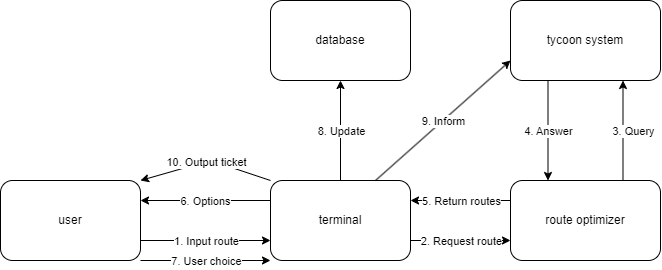
\includegraphics[width=\textwidth]{drawings/decision3_drawings/direct.png}
    \caption{Direct Data Management Interface}
    \label{fig:direct-data-interface}
\end{figure}

\subsection*{Option 2: Centralized Route Management Module}
A central route data management module acts as an intermediary between terminals and tycoon systems, standardizing and aggregating data before it is processed by the route optimizer. A database containing the timetables will be kept up to date by the tycoon (possibly though an API, this will be the focus of a later decision). The route data management system might cache optimized routes, in order to minimize database requests. A module specialized in running optimizations with the data it is provided with interacts solely with the Route Management Module.
\begin{figure}[ht]
    \centering
    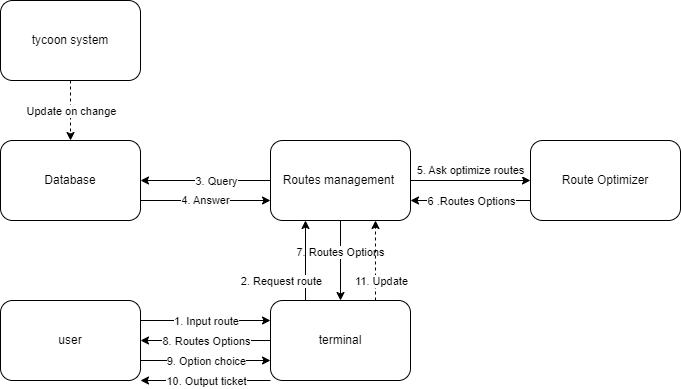
\includegraphics[width=\textwidth]{drawings/decision3_drawings/centralized.png}
    \caption{Centralized Route Management Module. Dashed lines represents steps to be explained in future decisions.}
    \label{fig:centralized-data-interface}
\end{figure}
  
\subsection*{Decision}
We have decided to proceed with Option 2: Centralized Route Management Module. This decision is based on the module's ability to simplify the data flow between systems and to effectively manage the complexity of integrating with multiple tycoon systems. The introduction of a separate data management module will allow for greater flexibility and scalability.

\subsection*{Consequences}
\textbf{Positive Consequences:}
\begin{itemize}
    \item Simplified data flow between the trip system and tycoons.
    \item Improved scalability and maintainability of the system.
    \item Easier to integrate with current and future tycoon systems.
\end{itemize}
\textbf{Negative Consequences:}
\begin{itemize}
    \item Initial development and integration effort for the new module.
    \item Potential complexity in data synchronization between modules.
\end{itemize}
This approach is expected to provide a solid foundation for the system's scalability and adaptability to evolving requirements and stakeholder needs.
\newpage
\subsection{Decision 4: Account and Subscriptions management}

\subsection*{Status}
Accepted.

\subsection*{Architectural Summary}


\subsection*{Concern}
A user wants to traver around the network using its subscription(s) instead of always having to buy a single fare.
Tycoons have explicitely requested to maintain their own subscriptions separated.
The following user stories are tied to this decision:
\begin{itemize}
    \item \textbf{User Story 16}: 16. As a passenger, I want to be able to purchase a single ticket that allows me to travel across all train networks so that I can travel seamlessly without needing to buy separate tickets for each tycoon's network.
    \item \textbf{User Story 23}: As a tycoon, I want the payment system to integrate with my existing infrastructure with minimal disruption so that I can maintain high service levels during the transition..
\end{itemize}

Specific concerns identified for the system include the following:
\begin{itemize}
    \item A passenger should be able to have different subscriptions for the three tycoons.
    \item Each of the three tycoon wants to have its own subscription fee system.
\end{itemize}

\subsection*{Context}
In developing the TrIP system, we explore subscription model architectures that align railway tycoons' need for flexibility with passengers' demand for simplicity. 
We assess the trade-offs between unified and tycoon-specific models to enhance both operational autonomy and passenger convenience.
When passengers want to go from station A to station B, they want to be able to use all the subscription they have and pay for the trains belonging to tycoons they are not subsribed to.
The terminal has to communicate with the tycoon systems to verify subscriptions and check routes.
Alternatively, if passengers have active subscriptions to a tycoon, they should be allowed onboard the train without a ticket. 

\subsection*{Criteria}
\begin{itemize}
\item Ease of use for the passenger.
\item Multiple route options for the user.
\item The system returns to user usable options based on price/time/availability/subscription.
\item Simple integration with the tycoon systems.
\end{itemize}

\subsection*{Option 1: Introduction of a subscription manager tool, route management needs to take subs into consideration.}
We want to include a Subscription Manager module to our functional view. 
Such a module has the responsibility to verify subscriptions, communicating with the tycoon system.
It should also allow users to create their own TRIP account and tie it to subscriptions.
Since we need scalability, we consider using a TRIP account that is tied to one or many subscriptions, and let the user add new or automatically renew the existing ones.
This means that we need an authentication means, like a magnetic card, or a phone app linked to NFC scanning or other alternatives.
This will be the topic of a future decision.
Furthermore, the Route management module needs to be able to optimize with respect to price, given that the passenger holds some subscription.
The idea is to add an optional initial iteration to the sequence of actions sketched in decision 3.
This requires a way to communicate the subscription to the terminal, be it a QR code, a code or a magnetic card. 
This should be the topic of another decision.

\subsection*{Pros}

\begin{itemize}[noitemsep]
    \item \textbf{Modular Architecture:} The separation of subscription management and route optimization into distinct modules enhances the system's modularity, making it easier to maintain, update, or replace parts of the system without affecting others.
    \item \textbf{Scalability:} Designed with scalability in mind, allowing for easy addition and management of new subscriptions or renewal of existing ones, which can accommodate growing user demands and evolving business requirements.
    \item \textbf{Reduced Risk of System-wide Failures:} By distributing functionalities across different systems or modules, the impact of a failure in one component is limited, reducing the risk of system-wide outages and improving overall system reliability.
    \item \textbf{Flexibility in User Authentication:} Supports various means of user authentication (e.g., magnetic card, smartphone app), offering flexibility and convenience for users to access their subscriptions and travel seamlessly.
\end{itemize}

\subsection*{Cons}

\begin{itemize}[noitemsep]
    \item \textbf{Increased System Interactions:} The decoupled nature of the system requires more interactions between separate modules (e.g., subscription verification and route optimization), which can increase the complexity of integration and potentially lead to higher latency in response times.
    \item \textbf{Integration Complexity:} Ensuring seamless communication and data consistency between different modules can introduce additional complexity in system integration and require more sophisticated coordination mechanisms.
    \item \textbf{Higher Overhead:} Managing separate systems for subscription and route optimization may lead to higher operational overhead in terms of both system resources and administrative efforts to maintain multiple components.
\end{itemize}
% The functional view schema is in my bag. TODO

\subsection*{Option 2: Integrated Subscription-Route Optimization Service}
The Integrated Subscription-Route Optimization Service (IS-ROS) combines the functionality of subscription management and route optimization into a single service. 
\subsubsection*{Pros}
\begin{itemize}[noitemsep]
    \item \textbf{Performance} Streamlines the process by combining two functionalities, potentially reducing response time for route optimization.
    \item \textbf{Reduced Interactions between systems} Simplifies the architecture by reducing the number of interactions between separate systems.
\end{itemize}
\subsubsection*{Cons}
\begin{itemize}[noitemsep]
    \item \textbf{Increased Complexity within Single Module} Increases complexity within a single system, which may require more resources to develop and maintain.
    \item \textbf{Failures have larger impact} May lead to higher dependency on a single system, which can be a point of failure if the system goes down.
\end{itemize}

\subsection*{Decision}
We decided to pick Option 1. The increased concern for scalability, caused by event 1, points clearly to the listed pros of this option. Furthermore, the focus on modularity
gives us easy maintenability, which is important for the TRIP owner.
Performance in this case doesn't seem to be that central, as optimization of routes should be precomputed and cached, given that timetables should not change often and that subscription have relatively long lasting periods.
With our option, we still have the flexibility to assign more computational or data access resources to the module who needs them the most.

\subsection*{Consequences}
\subsection*{Positive Consequences}

\begin{itemize}[noitemsep]
    \item \textbf{Enhanced Scalability:} Modular design facilitates easy scaling and integration of new features.
    \item \textbf{Improved Maintainability:} Simplifies updates and troubleshooting, allowing for technology-specific optimizations within each module.
    \item \textbf{Reduced System-wide Failure Risk:} Isolates failures to individual modules, enhancing overall system reliability.
\end{itemize}

\subsection*{Negative Consequences}

\begin{itemize}[noitemsep]
    \item \textbf{Increased System Complexity:} Necessitates sophisticated coordination and integration, potentially introducing latency.
    \item \textbf{Higher Initial Costs:} Development and maintenance of separate modules may lead to higher initial and operational costs.
    \item \textbf{Data Consistency Challenges:} Requires robust synchronization mechanisms to ensure data consistency across modules.
\end{itemize}


\newpage
\subsection{Decision 5: How to Handle Quickly Filling Trains?}

\subsection*{Status}
Accepted

\subsection*{Architectural Summary}
\textit{[Provide a brief summary of the architectural context and the specific system components affected by this decision.]}

\subsection*{Concern}
Ensuring a high level of usability and availability in the ticketing system is paramount. System operators and railroad tycoons aim to minimize customer service issues arising from passengers' frustrations with paying for unavailable routes.
\begin{itemize}
    \item \textbf{User Story 15}: Concerns about paying for unavailable routes.
    \item \textbf{User Story 26}: The need for real-time updates on train schedules.
    \item \textbf{User Story 27}: Integration with maintenance scheduling for minimal service disruption.
\end{itemize}

\subsection*{Context}
This decision seeks to address challenges associated with quickly filling trains, especially during peak hours, to offer a seamless and fair ticket purchasing experience. Mitigating the risk of overbooking and enhancing passenger satisfaction are central goals. It's critical to efficiently manage simultaneous requests for the last available seats to ensure a positive experience for commuters and students who rely on timely and available transportation.

\subsubsection*{QA scenario}
The following outlines a Quality Attribute (QA) scenario focusing on the real-time seat availability and booking process during peak hours. This scenario is structured to evaluate the system's usability and performance under conditions of high demand.
\paragraph{Source} Passenger interacting with a payment terminal (or any other way of booking tickets, e.g. an app or a website).
\paragraph{Stimulus} Two passengers try to buy the same ticket.
\paragraph{Artifact} The \textit{data management system}, \textit{database maintaining seat availability information} and the \textit{user interface} the passenger interacts with.
\paragraph{Response} Upon receiving the stimulus, the system's response is to immediately check the current availability of the selected seat, lock the seat for the passenger if it is available (thus preventing other bookings), and provide real-time feedback to the passenger regarding the seat's status (e.g., locked for purchase, already taken). If the seat is available and locked for the passenger, the system then proceeds with the payment process.
\paragraph{Response Measure}[\textit{After the decision is taken}] The effectiveness of the system's response is measured as follows:
\begin{itemize}
    \item Percentage of purchases ending with passengers buying the same ticket. This can be measured by a customer service.
\end{itemize}

\subsection*{Criteria}
\begin{itemize}
    \item Minimize excessive requests to tycoon systems, avoiding system overload.
    \item Ensure high performance to prevent a negative user experience.
    \item Prevent multiple users from paying for the same seat, ensuring fairness in ticket sales.
\end{itemize}

\subsection*{Option 1: Lock the Seats Before Payment}
We should maintain a database where info about scheduled trains is stored. This database should be updated by the terminal when a ticket has been bought. The database should ask periodically for updates on schedules from the tycoon systems. When a user selects that they want to pay for a specific ticket, that ticket should be locked, so that no one else can buy it. If the payment is not ultimated, it can be unlocked. Note that it can still happen that due to maintenance, a train is cancelled last minute. 

% TODO: What happens with the customer service? Should we add it to the context view? They will for sure need info from us, like who paid and how much. These should be two future decisions (how to deal with customer service in case of train disruptions, how to keep up to date about disruptions).

\subsubsection*{Pros}
\begin{itemize}[noitemsep]
    \item \textbf{Fairness} (Usability, Availability): Ensures that once a customer selects a ticket, it is reserved for them, preventing others from buying it.
    \item \textbf{Reduced System Load} (Performance, Efficiency): By locking seats before payment, it reduces the chances of multiple users attempting to pay for the same seat, thereby reducing system load.
\end{itemize}
\subsubsection*{Cons}
\begin{itemize}[noitemsep]
    \item \textbf{Potential for Seat Hoarding} (Usability, Efficiency): Customers might lock seats without completing the purchase, leading to temporarily reduced availability.
    \item \textbf{Increased Complexity} (Maintainability, Scalability): Managing locked seats, especially determining when to release them if payment is not completed, adds complexity.
\end{itemize}
\subsubsection*{User stories}
\begin{itemize}
    \item Directly addresses \textbf{User Story 15} by preventing payments for unavailable seats.
    \item Indirectly supports \textbf{User Stories 26 and 27} by contributing to system usability and reducing overbooking, though it does not directly offer real-time updates or integration with maintenance scheduling.
\end{itemize}

\subsection*{Option 2: Lock the Seats After Payment, FCFS, Refuse Payments if Seat is Booked}
Seats are locked only after payment confirmation, adhering to a first-come, first-served (FCFS) approach. This method ensures that seats are sold to passengers who complete the payment process first, minimizing the potential for holding seats unnecessarily.

\subsubsection*{Pros}
\begin{itemize}[noitemsep]
    \item \textbf{Efficiency} (Performance): Minimizes the time seats are unnecessarily held, as they are only locked upon payment completion.
    \item \textbf{Simplicity} (Maintainability): Easier to implement and maintain than preemptive locking mechanisms.
\end{itemize}
\subsubsection*{Cons}
\begin{itemize}[noitemsep]
    \item \textbf{User Experience} (Usability): Customers may go through the payment process only to find out the seat has been taken, leading to frustration.
    \item \textbf{Race Conditions} (Reliability): Higher risk of race conditions where multiple users complete payments for the last seat simultaneously.
\end{itemize}

\subsubsection*{User stories}
\begin{itemize}
    \item Aims to ensure fairness in seat allocation (\textbf{User Story 15}) by adhering to a first-come, first-served basis, reducing the risk of paying for unavailable seats.
    \item Does not directly address \textbf{User Stories 26 and 27}, but supports system performance and minimizes unnecessary seat holds.
\end{itemize}

\subsection*{Option 3: Real-time Seat Availability with Dynamic Allocation}
This option introduces a system for real-time tracking and dynamic allocation of seats. It involves continuous synchronization with tycoon systems to update seat availability instantly. The system could allow for a slight overbooking based on historical no-show rates, with safeguards in place to manage overbooked scenarios, such as offering alternative transportation options or compensation.

\subsubsection*{Pros}
\begin{itemize}[noitemsep]
    \item \textbf{Real-time Updates} (Availability, Usability): Enhances user experience by providing immediate feedback on seat availability.
    \item \textbf{Adaptability} (Scalability, Reliability): Can dynamically adjust to changing conditions, like cancellations or no-shows.
\end{itemize}
\subsubsection*{Cons}
\begin{itemize}[noitemsep]
    \item \textbf{Complex System Integration} (Maintainability, Operability): Requires continuous synchronization with external systems, increasing complexity.
    \item \textbf{Potential for Overbooking} (Usability, Reliability): While overbooking can be managed, it may lead to negative customer experiences.
\end{itemize}
\subsubsection*{User stories}
\begin{itemize}
    \item Directly solves \textbf{User Story 15}'s issue by ensuring passengers only pay for available seats and addresses \textbf{User Story 26} by providing real-time updates on train schedules.
    \item Supports \textbf{User Story 27} through dynamic allocation that can adjust to maintenance schedules, minimizing service disruptions.
\end{itemize}

\subsection*{Option 4: 2PC Protocol}
The Two-Phase Commit (2PC) protocol is a distributed transaction protocol that ensures all parts of a transaction across multiple systems either complete successfully or fail altogether. It is particularly useful in environments requiring strong consistency and atomicity, such as train terminal payment systems handling ticket purchases.

\subsubsection*{Pros}
\begin{itemize}[noitemsep]
    \item \textbf{Atomicity and Consistency} (Reliability, Consistency): 2PC guarantees that a transaction across distributed components either fully commits or fully aborts, maintaining the integrity and consistency of the database.
    \item \textbf{Fault Tolerance} (Availability, Reliability): By ensuring that all components agree on a transaction's outcome, 2PC enhances the system's ability to recover from partial failures without losing data integrity.
    \item \textbf{Coordination} (Integrity, Consistency): 2PC effectively coordinates complex transactions across multiple systems, ensuring that all parts of the transaction are synchronized.
\end{itemize}

\subsubsection*{Cons}
\begin{itemize}[noitemsep]
    \item \textbf{Performance Overhead} (Performance, Efficiency): The two-phase nature of the protocol can introduce latency, as it requires all participants to lock resources and wait for global commit or abort decisions.
    \item \textbf{Resource Locking} (Availability, Scalability): 2PC requires resources to be locked during the transaction, which can decrease system availability and limit scalability due to locking contention.
    \item \textbf{Complexity} (Maintainability, Operability): Implementing and maintaining a 2PC system introduces complexity, requiring robust failure and recovery mechanisms, and can complicate system operations and maintenance.
    \item \textbf{Risk of Blocking} (Availability): In cases where the coordinator fails after initiating the transaction but before completing it, participants can be left in a blocking state, waiting indefinitely for a decision and thus affecting system availability.
\end{itemize}
\subsubsection*{User stories}
\begin{itemize}
    \item Indirectly supports \textbf{User Story 15} by ensuring transactional integrity, which is foundational for reliable seat booking but does not directly address usability concerns.
    \item Does not directly address \textbf{User Stories 26 and 27}, but by ensuring consistent and reliable transactions, it lays the groundwork for future enhancements that could.
\end{itemize}

\subsection*{Decision}
In light of the trade-off analysis performed for each Option listed above, we decided to take Option 1. 
This Option ensures a solution to \textbf{User Story 15}, by effectively preventing two users to buy the same tickets. 
It is also good for reliability, a focus of the tycoons and for the usability required by the passengers, as they don't have to restart the booking procedure in case of failed payment.
Other options can lead to overbooking, which is unwanted given the concerns of passengers and tycoons.
Option 4 can be useful if the system is decentralized, but introduces unwanted complexity.

\subsection*{Consequences}
\textbf{Positive Consequences:}
\begin{itemize}
    \item Improved passenger experience through fair and efficient seat allocation.
    \item Reduced customer service issues related to overbooking and ticket availability.
    \item Enhanced system resilience against peak demand scenarios.
\end{itemize}
\textbf{Negative Consequences:}
\begin{itemize}
    \item Potential increase in system complexity and operational costs.
    \item Challenges in accurately forecasting demand for dynamic seat allocation or overbooking strategies.
    \item Possible passenger dissatisfaction in cases of overbooking or changes in train schedules.
\end{itemize}
\newpage
\subsection{Decision 6: Database scope and organization}

\subsection*{Status}
Review.

\subsection*{Architectural Summary}


\subsection*{Context}
We need to answer the following questions:
\begin{itemize}
\item Which info do we keep in the database? 
\item Do we need one or many databases?
\item How do we handle data protection?
\item How do we handle data update from tycoons/station management? (maybe for another decision?)
\end{itemize}

\subsection*{Concern}
We need to keep some information available from our system, but security of the data (especially payment and account data) is crucial for the government and for the passengers concerns.

\subsubsection*{User stories}
The following user stories are particularly relevant to the decision on the database scope, emphasizing the need for comprehensive management of subscriptions, security, and system integration:

\begin{itemize}[noitemsep]
    \item \textbf{User Story 1:} As a frequent traveler, I want to subscribe to a comprehensive monthly pass that includes all three networks so that I can save money on my regular commutes.
    
    \item \textbf{User Story 2:} As a passenger, I want to be able to check the balance of my multi-network travel card online so that I can easily manage my travel expenses.
    
    \item \textbf{User Story 3:} As a passenger with a subscription, I want to receive automatic notifications about my subscription renewal and any discounts or promotions available so that I can take advantage of cost savings. 
    
    \item \textbf{User Story 4:} As a tech-savvy passenger, I want to use a mobile app to manage my subscriptions, make payments, and receive digital tickets so that I can have a paperless and convenient travel experience. 
    
    \item \textbf{User Story 5:} As a passenger interested in sustainability, I want the system to track my travel carbon footprint and offer carbon offset options so that I can make environmentally responsible travel choices.
    
    \item \textbf{User Story 6:} As a passenger with mobility challenges, I want the payment system to provide information on accessible services and allow for easy purchase of accessible seating across all networks so that I can travel comfortably and safely.
    
    \item \textbf{User Story 16:} As a passenger, I want to be able to purchase a single ticket that allows me to travel across all train networks so that I can travel seamlessly without needing to buy separate tickets for each tycoon's network.
    
    \item \textbf{User Story 18:} As a government regulator, I want the payment system to adhere to data protection and financial transaction security standards so that passengers' personal and financial information is secure.
    
    \item \textbf{User Story 23:} As a tycoon, I want the payment system to integrate with my existing infrastructure with minimal disruption so that I can maintain high service levels during the transition.
    \item 
    \item \textbf{User Story 27:} As a network maintenance planner, I want the payment system to integrate with maintenance scheduling tools so that I can plan work with minimal disruption to the train service and revenue.
\end{itemize}

\subsection*{Option 1: Querying modules or external parties should know as little as possible}
We try to have one database for each important set of information that the system needs to know.
We try to stick to the Separation of Concerns principle, so that each module only has access to the data it scricly needs to operate.
We divide the following:
\begin{itemize}
    \item A database containing the timetable, the prices of seats and the bookings.
    \item A database containing the optimized routes cached after being calculated by the Routes Optimization Module.
    \item A database containing info about the accounts and their subscriptions. 
    \item A database recording payments that have been done, which should be accessed in case for example of complaints. 
\end{itemize}
\begin{figure}[ht]
    \centering
    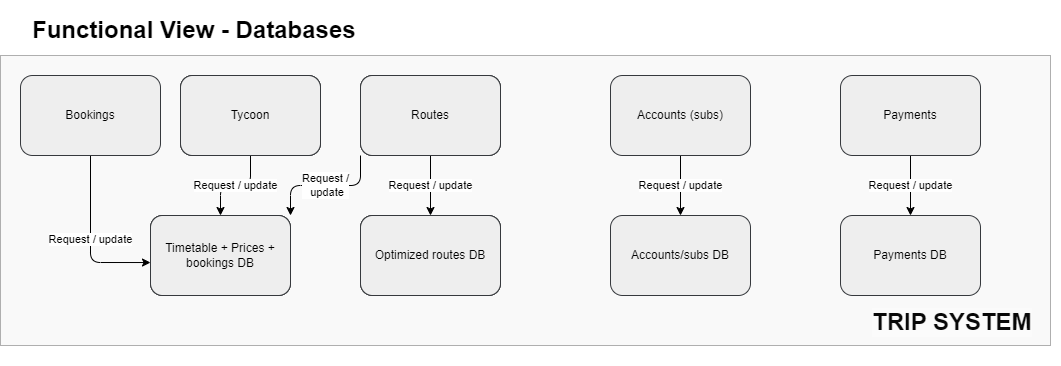
\includegraphics[width=\textwidth]{drawings/views_draft2/functional_view databases.png}
    \caption{Division of databases and their interaction with modules or stakeholders.}
    \label{fig:databases_view}
\end{figure}

\subsubsection*{Pros}
\begin{itemize}[noitemsep]
    \item \textbf{Enhanced Security} (Data Protection, Privacy): By segregating data across multiple databases, sensitive information is better protected, and access can be tightly controlled on a need-to-know basis.
    \item \textbf{Specialized Optimization} (Performance, Efficiency): Dedicated databases allow for optimization specific to their function, such as faster queries for timetable and booking data versus complex route optimization calculations.
\end{itemize}

\subsubsection*{Cons}
\begin{itemize}[noitemsep]
    \item \textbf{Increased Maintenance Overhead} (Maintainability, Complexity): Managing multiple databases adds complexity to the system's architecture, requiring more resources for maintenance and potentially higher costs.
    \item \textbf{Data Synchronization Challenges} (Reliability, Consistency): Ensuring data consistency across different databases can be challenging, especially in real-time, and may affect the system's overall reliability.
\end{itemize}

\subsection*{Option 2: Unified Centralized Database System}

This option proposes a centralized database architecture that consolidates all necessary information into a single, unified database system. It incorporates robust access control layers to manage data access based on module or user roles, ensuring that each part of the system accesses only the data it needs for operation. This model simplifies data management, enhances security through centralized control mechanisms, and facilitates easier updates and integrations. This model can be improved with having accounts database as a separate component, and keeping the rest of the databases central. In this way accounts data will be secure, and the rest of the systems will access accounts data anonymously via ids. Manage permissions for eacsh tycoon, on which info they can access (they shouldn't be able to connect name to bank account). In this way we can keep everything in the same place, but each tycoon api will have specificed access protocols. Tycoons can only update timetables and prices.

We can keep bookings data a DaaS, since it needs to be updated regularly and concurrently. Rest can be a server based database. Since we can cache routes we don't want cloud services for these. 

\subsubsection*{Pros}
\begin{itemize}[noitemsep]
    \item \textbf{Simplified Data Management} (Maintainability, Efficiency): Centralizing data storage simplifies the architecture by reducing the number of systems to manage, making it easier to maintain and update the database.
    \item \textbf{Improved Data Consistency} (Reliability, Integrity): A unified database ensures that all modules access the most current and consistent data, reducing the risk of discrepancies and errors.
    \item \textbf{Enhanced Integration Capability} (Scalability, Interoperability): With all data in one place, integrating new features, modules, or external systems becomes more straightforward, promoting scalability and interoperability.
\end{itemize}

\subsubsection*{Cons}
\begin{itemize}[noitemsep]
    \item \textbf{Risk of a Single Point of Failure} (Reliability, Availability): Centralizing data creates a single point of failure, which could potentially lead to system-wide outages affecting all functionalities if the database goes down.
    \item \textbf{Scalability Concerns} (Performance, Scalability): As the system grows, a centralized database might struggle with performance issues due to the increasing volume of data and concurrent access requests.
    \item \textbf{Complexity in Ensuring Data Protection} (Security, Privacy): Protecting a large, centralized repository of sensitive information poses significant challenges, requiring robust security measures to prevent unauthorized access and data breaches.
\end{itemize}

\subsection*{Option 3: Database per tycoon or not}

\subsubsection*{Pros}
\begin{itemize}[noitemsep]
    \item \textbf{Tycoon specific features} 
    \item \textbf{Tycoon access permissions are automatically managed} 
\end{itemize}

\subsubsection*{Cons}
\begin{itemize}[noitemsep]
    \item \textbf{Hard to manage the database} 
    \item \textbf{Shared data is potentially doubled} 
\end{itemize}

\subsection*{Option 4: Hybrid cloud storage}
Crucial data stored in cloud (timetables, and prices and bookings). Non-crucial data (accounts, payments) gets stored in non-cloud database one per tycoon, such that they can only access their own customer data.

\subsubsection*{Pros}
\begin{itemize}[noitemsep]
    \item \textbf{Tycoon specific access for accounts data} 
    \item \textbf{Secure and qucik access to data crucial data} 
    \item \textbf{Cheap storage for non-crucial data} 
\end{itemize}

\subsubsection*{Cons}
\begin{itemize}[noitemsep]
    \item \textbf{Can get expensive} 
    \item \textbf{Implementation of two different database types and their interactions setup}
\end{itemize}

\subsection*{Decision}
We choose Hybrid cloud storage System, increased Availability which is important for event 2 which requirees less stringent Maintainability and cost requirements. Cloud increased cost and interaction between databases increase Maintainability compared to single database.
\subsection*{Consequences}
\textbf{Positive Consequences:}
\begin{itemize}
    \item \textbf{database as a service}: Single point of failure is reduced, scalable.
    \item \textbf{}: Single point of failure is reduced, scalable.
\end{itemize}
\textbf{Negative Consequences:}
\begin{itemize}
    \item \textbf{Tycoon permission management} : More complextiy, we need to restrict access for each tycoon.
    \item \textbf{Single point of failure} : If database fails, everything fails.(bad for availablity)[maybe a solution is backup database].
    \item \textbf{database as a service}: Expensive.
\end{itemize}
\newpage
\subsection{Decision 7: Customer Service}

\subsection*{Status}
Open

\subsection*{Architectural Summary}

\subsection*{Concern}
The primary concern is to ensure that customer service representatives have access to accurate and timely information to address passenger queries and resolve issues efficiently, without compromising data privacy.

\subsection*{Context}
This decision outlines the strategy for communication between the TrIP system and customer service teams to facilitate rapid and effective resolution of customer issues.
Customer service teams require real-time access to passenger data, ticketing information, and system status to provide informed support. The chosen communication strategy must balance the need for information accessibility with system security and data privacy regulations.

\subsection*{Criteria}
\begin{itemize}
    \item Timeliness and accuracy of information communicated.
    \item Data privacy and security compliance.
    \item Ease of access for customer service representatives.
    \item Minimization of system complexity and maintenance.
    \item Integration with existing customer service platforms.
    \item Cost-effectiveness of the communication solution.
\end{itemize}

\subsection*{Option 1: Direct Access to Live Data}
Grant customer service representatives direct access to the live operational database with appropriate read-only permissions and privacy safeguards in place.

\subsection*{Option 2: Periodic Data Sync to a Dedicated Customer Service Database}
Regularly synchronize relevant data from the operational database to a separate customer service database designed for query efficiency and tailored access control.

\subsection*{Option 3: On-Demand Data Retrieval via Secure API}
Implement a secure API that allows customer service representatives to retrieve necessary data on-demand while maintaining strict access controls and audit trails.

\subsection*{Option 4: Automated Reporting System}
Develop an automated reporting system that provides customer service representatives with pre-defined reports and dashboards, reducing the need for direct data access.

\subsection*{Decision}
Option 3 is chosen: not enough requests to justify the burden of an additional db. option4 requires to much work from us. Option 1 doesnt seem secure enough.

\subsection*{Consequences}
\textbf{Positive Consequences:}
\begin{itemize}
    \item Option 1: Immediate access to data allows for quick customer service responses.
    \item Option 2: Data syncing provides a stable environment tailored for customer service needs.
    \item Option 3: Secure API ensures data privacy and minimizes unnecessary data exposure.
    \item Option 4: Automated reports streamline the information delivery process.
\end{itemize}
\textbf{Negative Consequences:}
\begin{itemize}
    \item Option 1: Direct access to live data could pose security risks if not managed correctly.
    \item Option 2: Data syncing could lead to delays in information relay if not frequent enough.
    \item Option 3: On-demand retrieval may introduce latency and requires robust API management.
    \item Option 4: Automated reporting may not cover all ad-hoc queries from customer service representatives.
\end{itemize}
% TODO: move options pros and cons to the options subsections.
\newpage
\section*{Decision 8: Serverless vs. Servers for calculations}

\subsection*{Status}

\subsection*{Architectural Summary}


\subsection*{Concern}


\subsection*{Context}


\subsection*{Criteria}
\begin{itemize}
\end{itemize}

\subsection*{Option 1: Serverless}
You dont deal with servers.

\subsection*{Option 2: Servers}
Data is not shared with third party.

\subsection*{Decision}

\subsection*{Consequences}
\textbf{Positive Consequences:}
\begin{itemize}
\end{itemize}
\textbf{Negative Consequences:}
\begin{itemize}
\end{itemize}
\newpage
\subsection{Decision 9: Account management and authentication}

\subsection*{Status}
Review
\subsection*{Architectural Summary}


\subsection*{Concern}
\subsubsection*{User stories}

\subsection*{Context}
\subsubsection*{QA Scenario} % not always needed I believe
\subsection*{Criteria}
% \begin{itemize}
% \end{itemize}

Get online account, how to open account (at terminal, online, app), how to make the turnstile/controller know that you have the account (anonymous card, bank card, nominal card, nfc).

\subsection*{Option 1: anonymous card}
\subsection*{Option 2: bank credit card}
Pay at the terminal
\subsection*{Option 3: phone app}
You can payonline and create accounts, you can scan qr code from the app or nfc (google wallet) at turnstiles.

\subsection*{Option 4: nominal card}
Pay at terminal, get account and card, scan it at turnstiles. Access online account via browser. (possibly mix with opt 3)

\subsection*{Option 5: NFC reader/google wallet}


\subsubsection*{User Stories}
\subsection*{Decision}
app (with nfc, connected to bank account) + fillable card (for tourists, anoymous) + physical nominal card.
Deciding to have everything can require a lot of work: is it justified?

We want to scan either credit cards or QR code at scanning devices:
    - bank plugin that gives an ID of the card (connected to account or not) 
    - qr code on a ticket / TRIP card / app generated / fillable card
% TODO: discussion about pros/cons and user stories, depending on given prios of stakeholders and previous decision.
\subsection*{Consequences}
\textbf{Positive Consequences:}
% \begin{itemize}
% \end{itemize}
\textbf{Negative Consequences:}
% \begin{itemize}
% \end{itemize}
\newpage
\subsection{Decision 9: Template}

\subsection*{Status}

\subsection*{Architectural Summary}


\subsection*{Concern}
\subsubsection*{User stories}

\subsection*{Context}
\subsubsection*{QA Scenario} % not always needed I believe
\subsection*{Criteria}
\begin{itemize}
\end{itemize}

\subsection*{Option 1: }

\subsection*{Decision}

\subsection*{Consequences}
\textbf{Positive Consequences:}
\begin{itemize}
\end{itemize}
\textbf{Negative Consequences:}
\begin{itemize}
\end{itemize}
\newpage
\subsection{Decision 11: How to interact with customer service?}

\subsection*{Status}

\subsection*{Architectural Summary}


\subsection*{Concern}
\subsubsection*{User stories}

\subsection*{Context}
\subsubsection*{QA Scenario} % not always needed I believe

\subsection*{Criteria}
\begin{itemize}
\end{itemize}

\subsection*{Option 1: }
\subsubsection*{User Stories}
\subsection*{Decision}
% discussion about pros/cons and user stories, depending on given prios of stakeholders and previous decision.
\subsection*{Consequences}
\textbf{Positive Consequences:}
\begin{itemize}
\end{itemize}
\textbf{Negative Consequences:}
\begin{itemize}
\end{itemize}
\newpage
\subsection{Decision 12: How to handle disruptions?}

\subsection*{Status}

\subsection*{Architectural Summary}


\subsection*{Concern}
\subsubsection*{User stories}

\subsection*{Context}
Which info do we keep in the database? 
Do we need more databases?
How do we handle data protection?
How do we handle data update from tycoons/station management? (maybe for another decision?)

\subsubsection*{QA Scenario} % not always needed I believe
Usability.
\subsection*{Criteria}
\begin{itemize}
\end{itemize}

\subsection*{Option 1: }

\subsection*{Decision}

\subsection*{Consequences}
\textbf{Positive Consequences:}
\begin{itemize}
\end{itemize}
\textbf{Negative Consequences:}
\begin{itemize}
\end{itemize}
\newpage
\subsection{Decision 13: Serverless vs. Servers for Calculations}

\subsection*{Status}
Open

\subsection*{Architectural Summary}
This decision examines the computational approach for the TrIP system, specifically whether to adopt a serverless architecture or to maintain dedicated servers for processing calculations related to ticketing, route optimization, and other system functionalities.

\subsection*{Concern}
The primary concern is to select a computational architecture that balances scalability, cost, performance, and data privacy for processing passenger data and transactional information.

\subsection*{Context}
The computational backbone of the TrIP system must handle variable workloads efficiently, especially during peak hours when route calculations and payment processing are at their highest demand. Additionally, the system must maintain data privacy and adhere to regulatory compliance.

\subsection*{Criteria}
\begin{itemize}
    \item Scalability to handle peak and off-peak loads.
    \item Cost-effectiveness, including operational and maintenance costs.
    \item Performance in terms of latency and throughput.
    \item Data privacy and control.
    \item Compliance with data protection and privacy laws.
    \item Ease of maintenance and updates.
\end{itemize}

\subsection*{Option 1: Serverless}
Adopting a serverless architecture where the service provider dynamically manages the allocation of machine resources.
\subsubsection*{Pros}
\begin{itemize}
    \item Cost efficiency during low usage.
    \item No need for server maintenance.
    \item Automatic scaling.
\end{itemize}
\subsubsection*{Cons}
\begin{itemize}
    \item Potential for increased latency.
    \item Less control over data.
    \item Possible security concerns.
\end{itemize}

\subsection*{Option 2: Dedicated Servers}
Using dedicated servers, either on-premises or hosted, to handle all computations.
\subsubsection*{Pros}
\begin{itemize}
    \item Greater control over data.
    \item Potentially better performance.
    \item Consistent availability.
\end{itemize}
\subsubsection*{Cons}
\begin{itemize}
    \item Higher upfront costs.
    \item Requires dedicated IT staff for maintenance.
    \item Might be underutilized during off-peak times.
\end{itemize}

\subsection*{Option 3: Hybrid Approach}
Implementing a hybrid system that uses a combination of serverless architecture for less sensitive and highly variable workloads, and dedicated servers for more predictable workloads and data-intensive tasks requiring stringent privacy controls.
\subsubsection*{Pros}
\begin{itemize}
    \item Balances the benefits of both serverless and dedicated servers.
    \item Provides scalability while maintaining data privacy for sensitive operations.
\end{itemize}
\subsubsection*{Cons}
\begin{itemize}
    \item Increased complexity in managing two different environments.
    \item Potential for higher operational costs.
\end{itemize}

\subsection*{Decision}
The decision will be based on a cost-benefit analysis of each option, considering the trade-offs between control, cost, and scalability. The chosen approach must align with the overall system requirements for performance, privacy, and regulatory compliance.

\subsection*{Consequences}
\textbf{Positive Consequences:}
% \begin{itemize}
% \end{itemize}
\textbf{Negative Consequences:}
% \begin{itemize}
% \end{itemize}

\newpage
\section{Context Viewpoint}

\subsection{Stakeholder Model}
\begin{figure}[H]
    \centering
    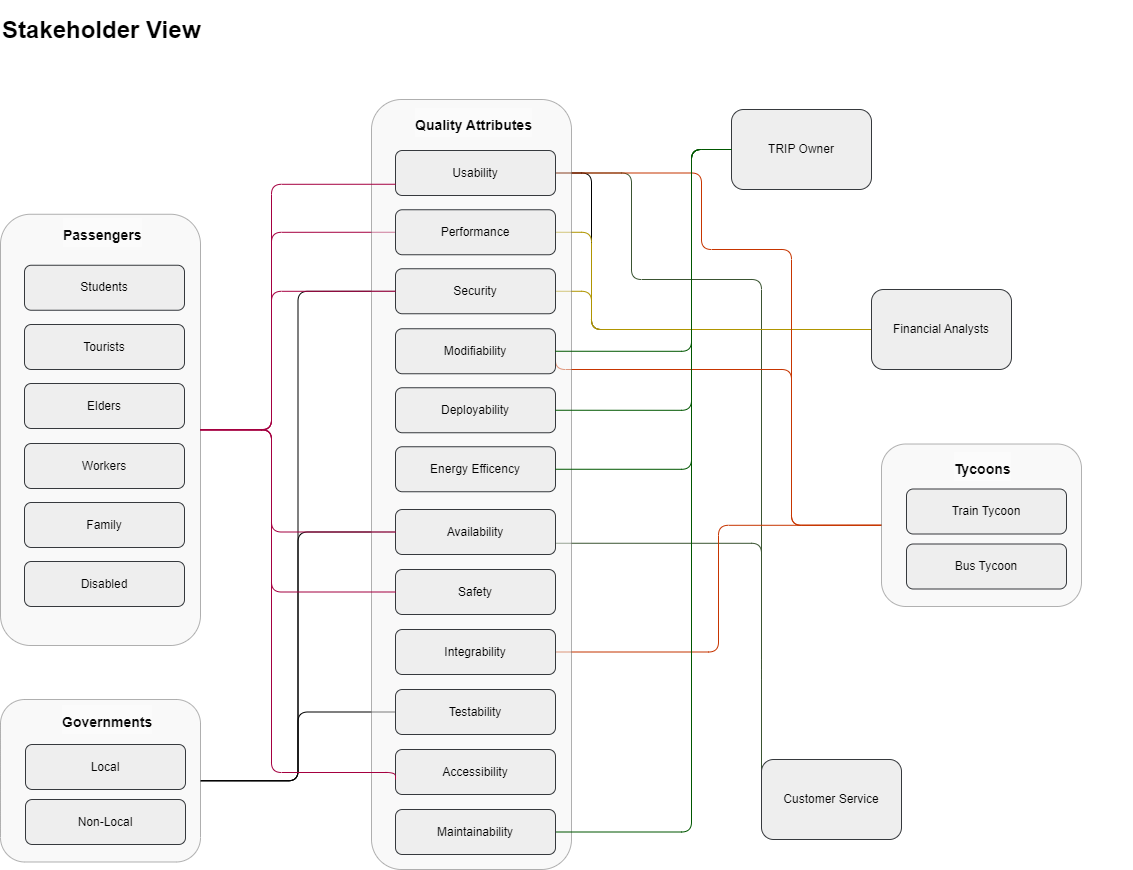
\includegraphics[width=\textwidth]{drawings/views_final_version/stakeholder_view.png}
    \caption{Stakeholder model of the TRIP system.}
    \label{fig:stakeholder_view_model}
\end{figure}

\subsection{Context Model}
\begin{figure}[H]
    \centering
    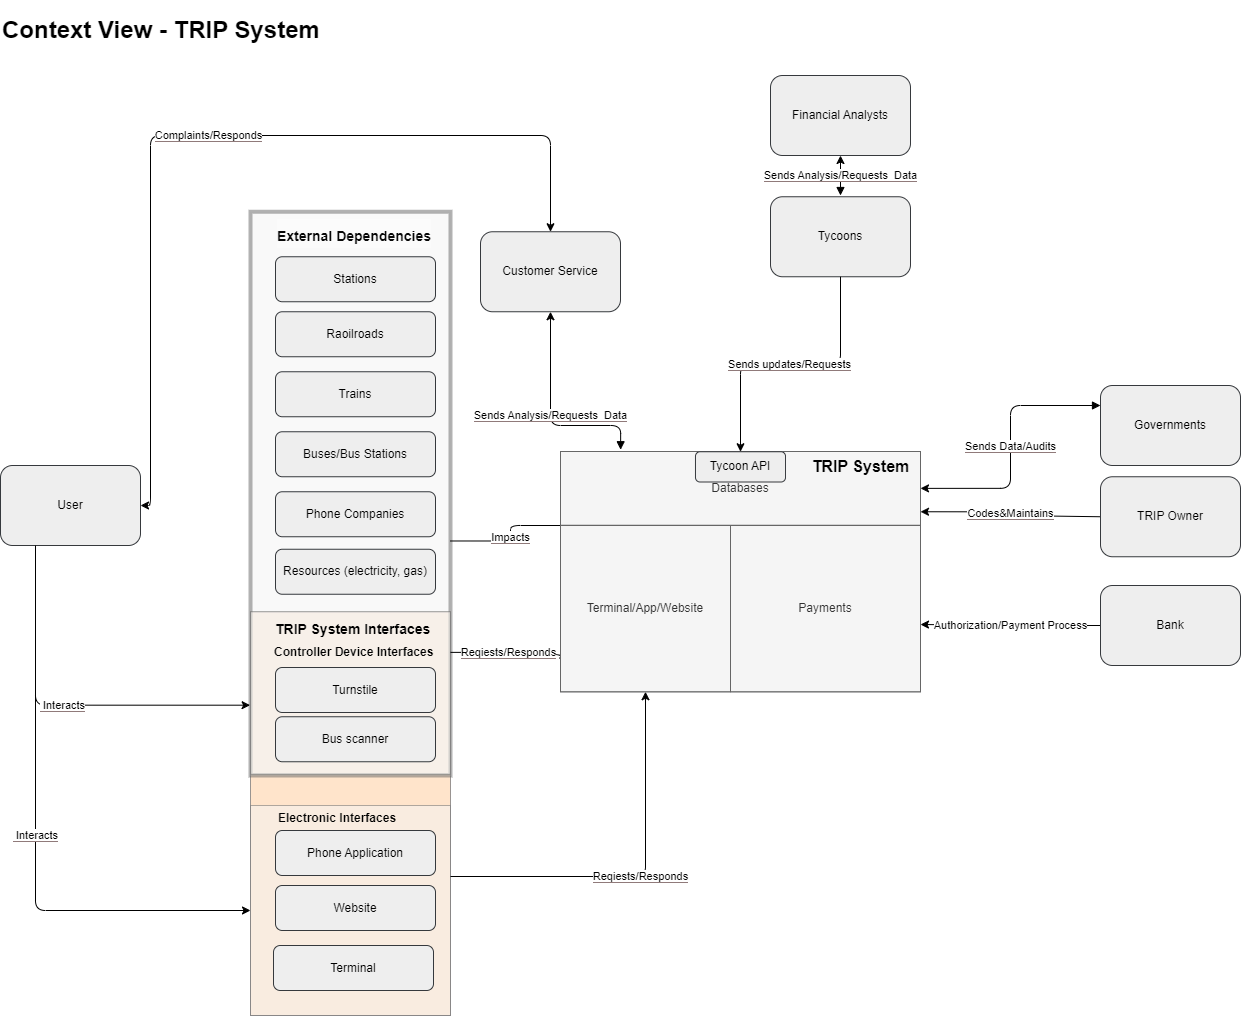
\includegraphics[width=\textwidth]{drawings/views_final_version/context_view.png}
    \caption{Context model of the TrIP system.}
    \label{fig:context_view_model}
\end{figure}

\subsection*{Description}
The Context View of the TRiP SYSTEM delineates the ecosystem within which the system operates, including its interactions with users, external entities, and other system components. At the user level, engagement with the TRiP system is facilitated through various interfaces such as terminals, apps, websites, and controller devices like turnstiles and bus scanners, enabling passengers to access services seamlessly.

The system is subject to a range of external dependencies, including infrastructure elements like stations, railroads, and trains, as well as service providers such as phone companies and utilities that supply essential resources. These components are integral to the system's operations, impacting its functionality and performance.

At the core, the TRiP system is interconnected with Tycoons via the Tycoon API, through which data flows bidirectionally, allowing for the exchange of updates, requests, and analytical data. The databases within the system are pivotal in managing schedules, user accounts, tickets, and payments, all of which are crucial for the day-to-day operations.

The system's architecture is designed to ensure robustness and responsiveness to both the passengers' and Tycoons' needs. It facilitates various processes, from payment transactions, which are securely handled and routed through financial institutions, to the maintenance of service quality, overseen by the TRiP owner and regulated by governmental audits and codes. This comprehensive network of interactions defines the TRiP system's context, emphasizing its multifaceted nature and the critical role it plays in serving its stakeholders.

\begin{table}[H]
\centering
\begin{tabular}{@{}clp{9cm}@{}}
\toprule
\textbf{Id} & \textbf{Name} & \textbf{Description} \\
\midrule
1 & Passenger & Individuals who use the TrIP SYSTEM and its associated services, interacting through various interfaces. \\
2 & Customer Service & The department that handles passenger complaints and feedback, providing support and sending analysis or data requests to the system. \\
3 & Financial Analysts & Experts or entities that review financial data, requiring analytical information from the system for decision-making. \\
4 & Tycoons & The operational decision-makers of the system, possibly managers or algorithms that control system parameters and require data. \\
5 & Tycoon API & The programming interface through which Tycoons receive updates and send requests to the system. \\
6 & TrIP System & The core system that integrates various interfaces and processes, forming the central operation platform. \\
7 & Governments & Regulatory bodies that may require data or perform audits on the system for governance and compliance. \\
8 & TrIP Owner & The entity or person owning and maintaining the TrIP SYSTEM, responsible for its overall functionality. \\
9 & Bank & Financial institution that handles the authorization and processing of payments for the system. \\
10 & Stations & Locations where the TrIP SYSTEM provides service to passengers, such as train or bus stations. \\
11 & Railroads & Infrastructure providers that offer the tracks on which train services operate. \\
12 & Trains & The vehicles used by the system to transport passengers from one station to another. \\
13 & Buses/Bus Stations & The bus services and their stations that are part of the transport network. \\
14 & Phone Companies & Telecom service providers that facilitate mobile communication and data transfer for the system. \\
15 & Resources (electricity, gas) & Utility providers that supply essential power and energy required for the system’s operations. \\
16 & Controller Device Interfaces & The interfaces like turnstiles and bus scanners that manage access control and validate user credentials. \\
17 & Electronic Interfaces & Digital platforms such as mobile applications and websites that passengers interact with for services. \\
\bottomrule
\end{tabular}
\caption{Context model glossary for the TrIP System.}
\label{tab:glossary_context_view}
\end{table}

\section{Functional Viewpoint}
\begin{figure}[H]
    \centering
    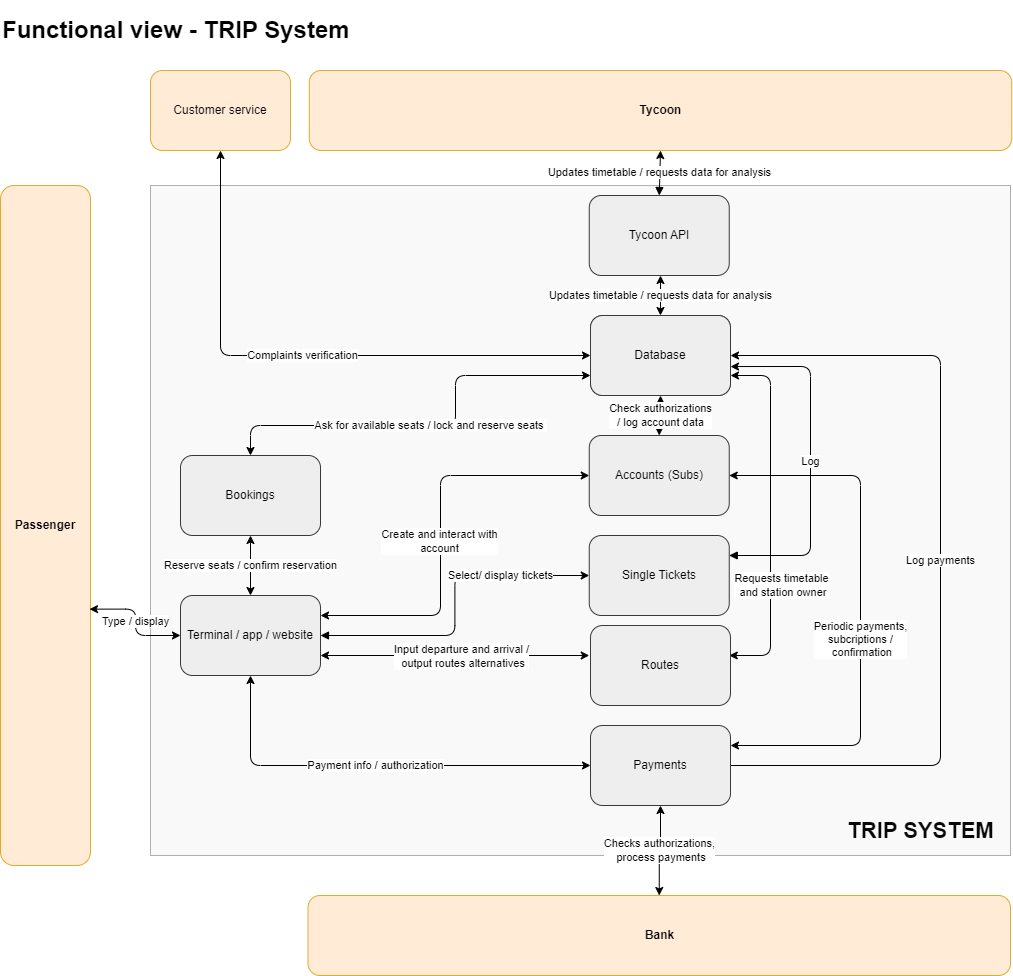
\includegraphics[width=\textwidth]{drawings/views_final_version/functional_view.png}
    \caption{TrIP System.}
    \label{fig:trip_system}
\end{figure}

\subsection*{Description}
The functional view diagram of the TrIP system illustrates the major functions of the system and how they interact with each other. The diagram features boxes representing different functions, connected by arrows that represent interactions.
The system starts with the user, who can interact with the system through various interfaces, such as terminals, apps, or websites. The user can input their departure and arrival stations, and the system will then display a list of available routes. The user can then select a route and proceed to payment.
The payment system can handle various payment methods, including single tickets, subscriptions, and fillable cards. If the user has a subscription, the system will automatically check if the subscription is valid for the selected route. This is done by the Account and Subscription Management module, which communicates with the tycoon systems to verify the subscription. If the subscription is not valid, the user will be prompted to purchase a single ticket or top up their fillable card.
Once the payment is processed, the system will generate a ticket or update the user's travel card. The user can then scan their ticket or card at the turnstile to gain access to the train platform. The turnstile communicates with the Account and Subscription Management module to verify the ticket or card and update the passenger's state.
The system also includes a number of other functions, such as a booking system, a route optimization system, and a customer service system. The booking system allows users to reserve seats on trains. The route optimization system helps users find the most efficient routes between their departure and arrival stations. The customer service system provides support to passengers with inquiries and complaints.
The system is designed to be scalable and flexible, so that it can be easily adapted to accommodate new tycoons and changing business models. The system is also designed to be secure, so that passenger data is protected from unauthorized access.

\begin{table}[H]
    \centering
    \begin{tabular}{@{}clp{9cm}@{}}
    \toprule
    \textbf{Id} & \textbf{Name} & \textbf{Description} \\
    \midrule
    1 & Passenger & End-users of the TrIP SYSTEM who interact with various system components to manage their travel experience. \\
    2 & Customer Service & The interface for passengers to make inquiries or complaints and receive assistance with bookings or account issues. \\
    3 & Tycoon & The administrative or business logic module that updates timetables and analyzes system data for improvements or reporting. \\
    4 & Database & An abstraction for the set of databases that stores all system data including passenger accounts, bookings, and payment information. Detailed information about how different databases are handled is detailed in the Information View.\\
    5 & Bookings & The system component where passengers can inquire about seat availability and make reservations. \\
    6 & Accounts (Subs) & The system managing passenger accounts and subscriptions, responsible for authorization checks and account data logging. 
    It is is also responsible for single tickets and fillable cards, as they can be seen as temporary and anonymous accounts. \\
    7 & Routes & The component that manages route information and provides passengers with timetables, station ownership details, and route alternatives. \\
    8 & Payments & The module handling all financial transactions, including passenger payments and periodic billing. \\
    9 & Bank & The financial institution interface for authorizing and processing payments linked to the system. \\
    10 & Terminal/App/Website & User interfaces through which they can access services such as booking, route information, and payment. \\
    \bottomrule
    \end{tabular}
    \caption{Glossary of elements detailing the components of the TrIP SYSTEM and their roles in facilitating user interaction and service provision.}
    \label{tab:glossary_trip_system}
\end{table}

\begin{figure}[H]
    \centering
    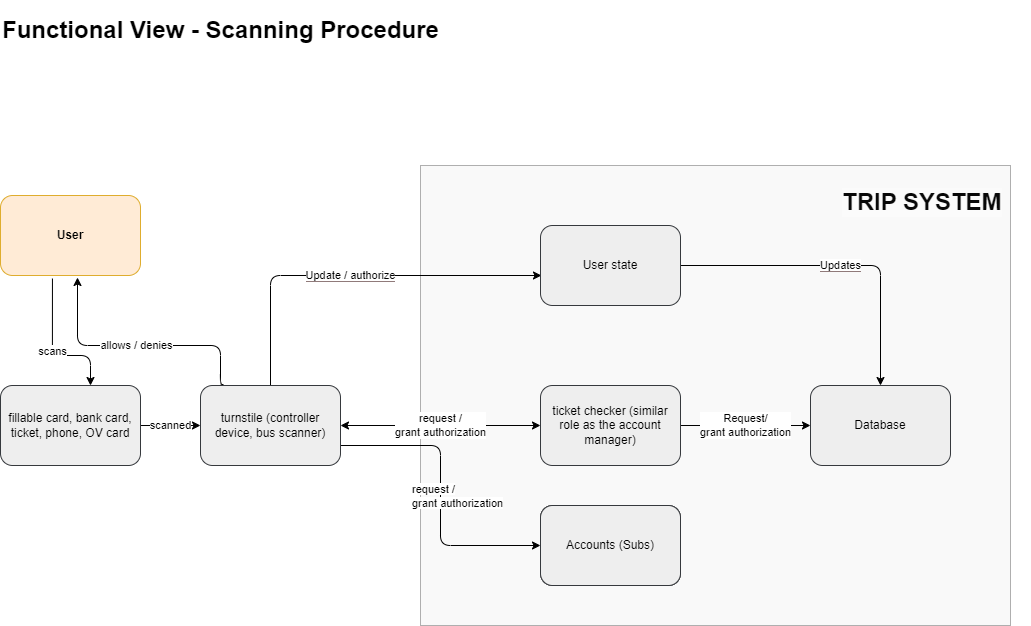
\includegraphics[width=\textwidth]{drawings/views_final_version/functional_view scanning.png}
    \caption{Interaction with a ticket scanner.}
    \label{fig:ticket_scanner}
\end{figure}

\subsection*{Description}
The scanning procedure within the TRIP SYSTEM encapsulates the interactions between the passenger and the system's access control mechanisms. It begins with the user presenting a valid form of transit access—such as a card or mobile device—to a scanning device like a turnstile or bus scanner. This device then consults the User state, a repository of the passenger's authorization status, to allow or deny entry. In parallel, the Ticket Checker function verifies the user's credentials against the Accounts subsystem, which manages detailed account information and subscriptions. Any changes to the user's status are updated in real time in the central Database, ensuring accurate tracking of access and travel history. This process ensures a secure, streamlined experience for passengers while providing the system with the necessary oversight to prevent unauthorized access

\begin{table}[H]
    \centering
    \begin{tabular}{@{}clp{9cm}@{}} % Adjust the width of the description column as needed to fit the page
    \toprule
    \textbf{Id} & \textbf{Name} & \textbf{Description} \\
    \midrule
    1 & Passenger & The individual who uses the trip system and interacts with various components such as turnstiles and ticket checkers. \\
    2 & Fillable Card, Bank Card, Ticket, Phone, OV Card & Various forms of identification or payment methods that the passenger can use within the system. These are scanned by the turnstile to allow or deny access. \\
    3 & Turnstile (Controller Device, Bus Scanner) & A physical barrier or scanner that reads the passenger's ticket or card and determines whether to grant or deny access based on the passenger state or account information. \\
    4 & Passenger State & A system component that maintains the current state of the passenger within the system, including authorization and access rights, which is updated upon passenger interaction with the turnstile. \\
    5 & Ticket Checker (Account Manager) & An agent or system role similar to the account manager that requests or grants authorization for passenger access, potentially by checking the passenger state against the database. \\
    6 & Accounts (Subs) & The subsystem managing passenger accounts and subscriptions, which may interact with the turnstile and ticket checker to verify and update passenger access rights. \\
    7 & Database & An abstraction for the set of databases that stores all system data including passenger accounts, bookings, and payment information. Detailed information about how different databases are handled is detailed in the Information View.\\
    \bottomrule
    \end{tabular}
    \caption{Glossary of elements for the Functional View - Turnstiles, detailing the components and their roles in passenger access and authorization within the TrIP SYSTEM.}
    \label{tab:glossary_turnstiles}
\end{table}

\subsection{Analysis on Perspectives}

\begin{table}[h!]
    \centering
    \resizebox{\textwidth}{!}{%
    \begin{tabular}{|l|c|c|c|c|c|c|c|c|c|}
      \hline
      & Usability & Performance & Security & Modifiability & Cost Efficiency & Availability & Safety & Integrability & Maintainability \\
      \hline
      Functional View & 
      \cellcolor{gray!60}X & % Usability (2nd priority)
      \cellcolor{gray!30}X & % Performance (3rd priority)
      & & 
      \cellcolor{gray!55}X & % Cost (3rd priority)
      \cellcolor{gray!15}X & % Availability (4th priority)
      & & 
      \cellcolor{gray!90}X \\ % Maintainability (1st priority)
      \hline
    \end{tabular}
    }
    \caption{Functional View Prioritized Quality Attributes}
    \label{tab:functional_view}
\end{table}

\subsubsection{Scenarios}
% Scenario 1: Usability Enhancement through Standardized UIs
\begin{table}[H]
    \centering
    \begin{tabularx}{\textwidth}{@{} lX @{}}
    \toprule
    \textbf{Aspect} & \textbf{Details} \\
    \midrule
    Source & Passenger interacts with the payment terminal UI. \\
    Stimulus & The passenger navigates the options to buy a ticket. \\
    Artifact & Standardized User Interface (UI) of the payment terminal. \\
    Response & The UI displays a clear, consistent, and intuitive navigation path for ticket purchase. \\
    Measure & 95\% of passengers successfully purchase tickets without assistance. \\
    \bottomrule
    \end{tabularx}
    \caption{Scenario for Usability - Standardized UIs}
    \label{table:usability_enhancement}
\end{table}


% Scenario 2: Scalability via Tycoon API
\begin{table}[H]
    \centering
    \begin{tabularx}{\textwidth}{@{} lX @{}}
    \toprule
    \textbf{Aspect} & \textbf{Details} \\
    \midrule
    Source & A new tycoon's system attempting to integrate with the TrIP system. \\
    Stimulus & The tycoon sends a request to access route and fare data. \\
    Artifact & Tycoon API that standardizes data exchange with the TrIP system. \\
    Response & The API facilitates the integration, providing access to the required data. \\
    Measure & Integration is completed within 3 business days, with zero errors in data format conversion. \\
    \bottomrule
    \end{tabularx}
    \caption{Scenario for Scalability via Tycoon API}
    \label{table:scalability_tycoon_api}
\end{table}

% Scenario: Payment Flexibility for Diverse User Groups
% Scenario: Accommodating Varied Payment Preferences
\begin{table}[H]
    \centering
    \begin{tabularx}{\textwidth}{@{} lX @{}}
    \toprule
    \textbf{Aspect} & \textbf{Details} \\
    \midrule
    Source & Passengers with varying preferences for payment, each approaching the transit system's access points. \\
    Stimulus & Passengers select their payment method of choice, ranging from physical cash for single rides to digitally managed subscriptions, and some opt for the convenience of pre-loaded fare cards. \\
    Artifact & Integrated payment and authentication platform within the TrIP system. \\
    Response & The system adeptly manages the assortment of transactions, crediting cash payments, verifying subscription validity, and debiting pre-loaded cards, all in a streamlined fashion. \\
    Measure & The system consistently processes transactions of all types with a rapid response rate, registering a less than 2-second average processing time and maintaining a transaction success rate of 99\%. \\
    \bottomrule
    \end{tabularx}
    \caption{Scenario for Usability via Accommodating Varied Payment Preferences}
    \label{table:varied_payment_preferences}
\end{table}

In addressing the Quality Attribute (QA) priorities highlighted by users, our functional viewpoint incorporates several key decisions designed to enhance usability, maintainability, scalability, and performance efficiency.

To meet the usability needs of users, we have opted for standardized User Interfaces (UIs). These UIs, being open-source and widely utilized, benefit from a large user base that contributes to their maintenance and robustness. This choice ensures a user-friendly and reliable interface for passengers over the long term. Furthermore, it aligns with the TrIP owner's preferences by offering ease of maintenance and low operational costs.

The introduction of multiple payment methods, including fillable cards, credit cards, and single tickets, significantly simplifies passenger interaction with the TrIP system. The integration of accounts and subscriptions further facilitates seamless travel across multiple tycoon networks, enabling passengers to efficiently manage and use their subscriptions.

In response to Event 1, which underscored the need for easier integration of new tycoons, we have implemented the Tycoon API. This API standardizes data requests from each tycoon, irrespective of their mode of transportation, thus facilitating the smooth integration of new tycoons into the system. The Tycoon API, in conjunction with the accounts and bookings module, ensures that passengers can effortlessly utilize their subscriptions across different networks and book their preferred routes.

Event 3, which focused on traffic jams, raised the importance of optimizing system performance during peak periods. By deciding on a centralized route management module, we have streamlined data flow between the TrIP system and the tycoons. This module not only simplifies data management but also enhances the system's ability to handle high request volumes through optimization and caching strategies.

In summary, the functional viewpoint of our system meticulously addresses the initial QA priorities, along with the challenges presented by new tycoon integration (Event 1) and traffic jams (Event 3). These decisions collectively ensure a user-friendly, scalable, and high-performing TrIP system for passengers, tycoons, and the TrIP owner alike.




\section{Information Viewpoint}

\begin{figure}[H]
    \centering
    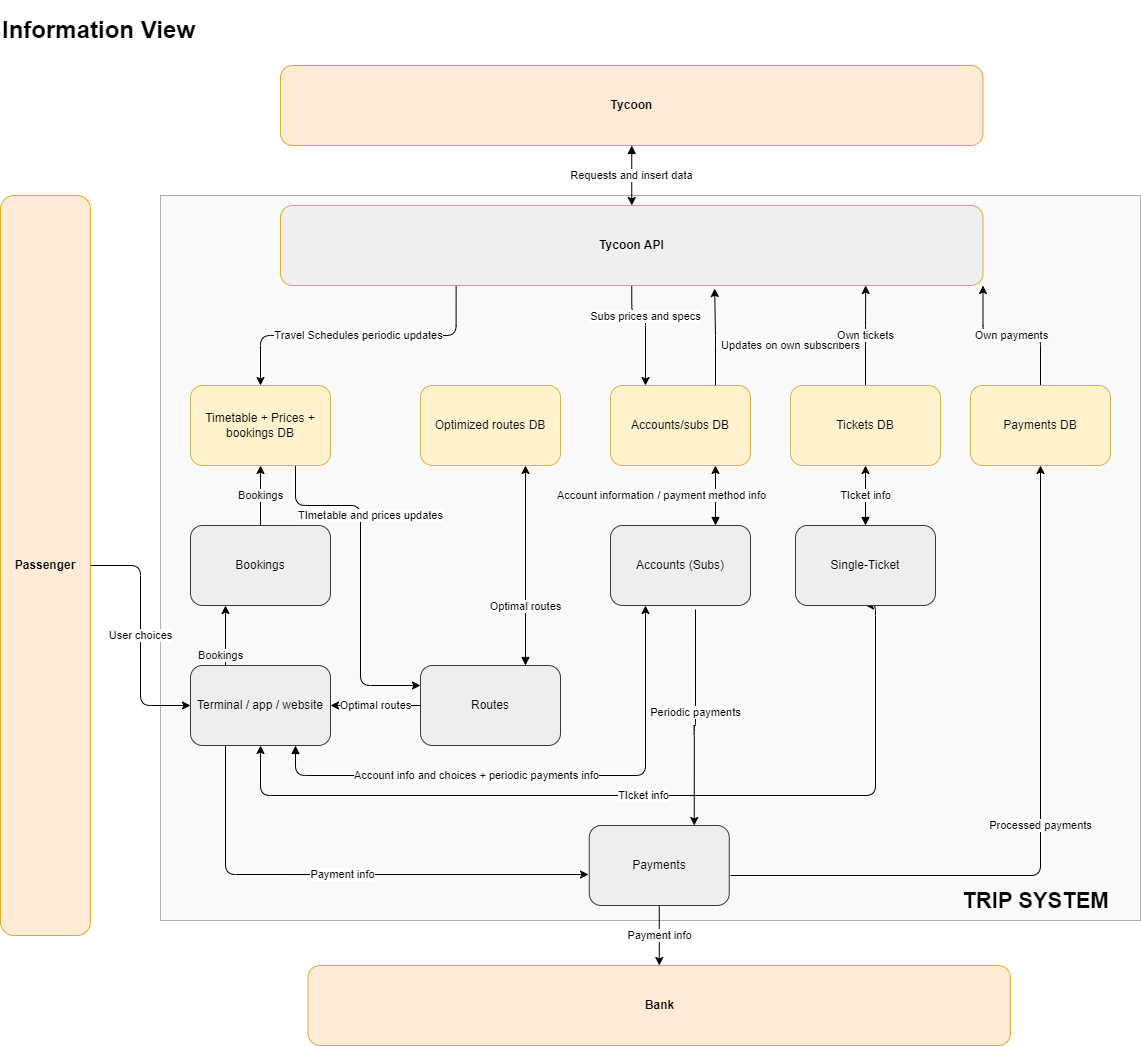
\includegraphics[width=\textwidth]{drawings/views_final_version/information_view.png}
    \caption{Information view.}
    \label{fig:information_view}
\end{figure}

\subsection*{Description}
The Information View of the TrIP SYSTEM is about how data moves and is stored. The system uses several databases. The Timetable + Prices + Bookings DB keeps track of schedules, prices, and reservations. The Optimized Routes DB has data on the best travel paths. The Accounts/Subs DB holds information on user accounts and subscriptions. The Tickets DB records ticket purchases, and the Payments DB keeps a record of all payments.

Tycoons use the Tycoon API to put in and get data. Passengers use terminals, apps, or websites to book travel and select routes. This choice and payment info go into the databases, updating the system.

The Routes component uses the Optimized Routes DB to give passengers the best travel options. The Accounts (Subs) part handles subscription details and payments, working with the Accounts/Subs DB. For single tickets, there's a separate interface that works with the Tickets DB. Payments process transactions and send completed payment information to the bank.

\begin{table}[H]
    \centering
    \caption{Glossary of elements for the Information View of the TrIP SYSTEM.}
    \label{tab:information_view_glossary}
    \begin{tabularx}{\textwidth}{@{}lX@{}} % Use 'X' for auto-adjusting width
    \toprule
    \textbf{Element} & \textbf{Description} \\
    \midrule
    Tycoon & Tycoons responsible for making requests for analysis, and inserting travel data. \\
    Tycoon API & Tycoon's way of interacting to the TrIP system. \\
    Timetable + Prices + bookings DB & Stores data regarding travel schedules, pricing, and booking information. \\
    Optimized routes DB & Contains information on the most efficient travel routes that have been calculated and stored. \\
    Accounts/Subs DB & Maintains records of user accounts and their subscriptions for travel services. \\
    Tickets DB & A database that logs ticket purchases and holds ticket-related information. \\
    Payments DB & Records and processes transactions related to payments within the system. \\
    Passenger & The end-user or customer who utilizes the system for travel services. \\
    Bookings & The system component or interface that passengers interact with to manage and view their bookings. \\
    Terminal / App / Website & The various platforms through which passengers can access the system for services. \\
    Routes & Involves the determination and selection of travel routes within the system. \\
    Accounts (Subs) & Manages the subscription details associated with user accounts. \\
    Single-Ticket & A system or interface that deals with the purchase of individual travel tickets. \\
    Periodic payments & Manages recurring payments, typically for subscription services. \\
    Payments & Processes transactions related to immediate payments within the system. \\
    Processed payments & A log or record of payment transactions that have been completed. \\
    Bank & The financial institution where final payment transactions are processed and funds are transferred. \\
    \bottomrule
    \end{tabularx}
\end{table}

\begin{figure}[H]
    \centering
    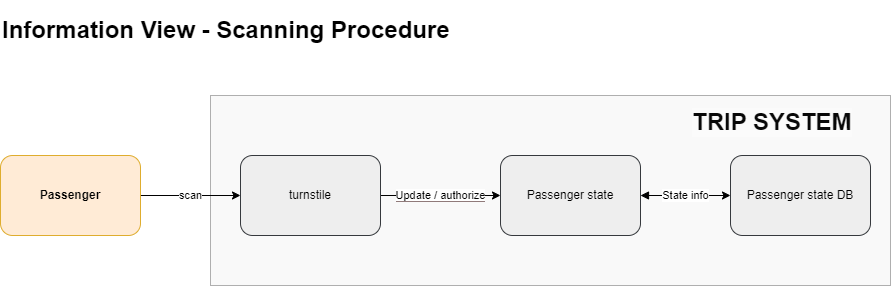
\includegraphics[width=\textwidth]{drawings/views_final_version/information_view scanning.png}
    \caption{Information view related to the scanning procedure.}
    \label{fig:information_view_scanning}
\end{figure}

\subsection*{Description}
The TrIP SYSTEM's scanning procedure is a sequence that starts with the Passenger, who scans at the Turnstile to gain entry. This triggers the Update/Authorize process, updating the Passenger State with the user's access rights. The Passenger State reflects the user's current permissions within the TRIP SYSTEM. Each user’s information is recorded in the Passenger State DB, a database that tracks and manages user statuses.

\begin{table}[H]
    \centering
    \caption{Legend for the Scanning Procedure in the Information View of the TrIP SYSTEM.}
    \label{tab:scanning_procedure_legend}
    \begin{tabular}{@{}llp{10cm}@{}}
    \toprule
    \textbf{Id} & \textbf{Name} & \textbf{Description} \\
    \midrule
    1 & Passenger & The starting point representing the individual using the TrIP SYSTEM. \\
    2 & Turnstile & The physical or virtual entry point where the passenger scans to gain access. \\
    3 & Update / Authorize & The process that updates the system and authorizes the passenger to proceed. \\
    4 & Passenger State & The current status of the passenger within the system, which is updated after scanning. \\
    5 & Passenger State DB & The database that records the state information of the passenger. \\
    \bottomrule
\end{tabular}
\end{table}

\subsection{Analysis on Perspectives}
\begin{table}[h!]
    \centering
    \resizebox{\textwidth}{!}{%
    \begin{tabular}{|l|c|c|c|c|c|c|c|c|c|}
      \hline
      & Usability & Performance & Security & Modifiability & Cost Efficiency & Availability & Safety & Integrability & Maintainability \\
      \hline
      Information View & 
       & % Usability
       & % Performance
      \cellcolor{gray!90}X & % Security (1st priority)
       & % Modifiability
       & % Cost Efficiency
       & % Availability
       & % Safety
       & % Integrability
       \\ % Maintainability
      \hline
    \end{tabular}
    }
    \caption{Information View Prioritized Quality Attributes}
    \label{tab:information_view}
\end{table}

\subsubsection{Scenarios}
% Scenario: Protecting Passenger Personal and Travel Information
\newcommand{\scenarioOneInformation}{
\begin{table}[H]
    \centering
    \begin{tabularx}{\textwidth}{@{} lX @{}}
    \toprule
    \textbf{Aspect} & \textbf{Details} \\
    \midrule
    Source & Passenger utilizing the TrIP system to manage their travel plans. \\
    Stimulus & The passenger enters personal and travel data into the system. \\
    Artifact & Encrypted Account Lookup Database within the TrIP system. \\
    Response & The system securely stores the passenger's data using state-of-the-art encryption both at rest and in transit, ensuring that personal and travel information is not accessible by unauthorized entities. Access to this data is restricted to specific operations within the TrIP system that require passenger verification. \\
    Measure & Passenger data breaches are non-existent, and passengers report a high level of trust in the system's data protection capabilities. Security logs show no unauthorized access, affirming the integrity of the encryption measures. \\
    \bottomrule
    \end{tabularx}
    \caption{Scenario for Security - Passenger Data Protection}
    \label{table:passenger_data_security}
\end{table}
}

% Scenario: Secure Payment Processing for Passenger Transactions
\newcommand{\scenarioTwoInformation}{
\begin{table}[H]
    \centering
    \begin{tabularx}{\textwidth}{@{} lX @{}}
    \toprule
    \textbf{Aspect} & \textbf{Details} \\
    \midrule
    Source & Passenger making a payment through the TrIP system. \\
    Stimulus & The passenger chooses a payment method and initiates a transaction. \\
    Artifact & Bank interfaced with TrIP system for processing payments. \\
    Response & The bank processes the payment with rigorous security protocols, ensuring that the payment information is handled in a secure, encrypted channel. The system guarantees that payment data is never stored within the TrIP system and is managed exclusively by the bank, providing an additional layer of security. \\
    Measure & Payment transactions are completed with zero incidents of data compromise, and the response time for transaction completion remains within 3 seconds. Post-transaction audits confirm the absence of payment data retention within the TrIP system. \\
    \bottomrule
    \end{tabularx}
    \caption{Scenario for Security - Secure Payment Transactions}
    \label{table:payment_transaction_security}
\end{table}
}

% Scenario: Controlled Access to Passenger Account Data
\newcommand{\scenarioThreeInformation}{
\begin{table}[H]
    \centering
    \begin{tabularx}{\textwidth}{@{} lX @{}}
    \toprule
    \textbf{Aspect} & \textbf{Details} \\
    \midrule
    Source & Passenger subscribing to a specific tycoon's services within the TrIP system. \\
    Stimulus & The subscribed tycoon requests access to the passenger's account data for service personalization. \\
    Artifact & Tycoon API enabling access control to passenger data within the TrIP system. \\
    Response & The TrIP system authenticates the tycoon's request through the Tycoon API, which validates that only the tycoon with whom the passenger is subscribed can retrieve the required data. This ensures that each tycoon can access only their passengers’ data, thus maintaining strict data access control and privacy. \\
    Measure & Regular audits indicate 100\% compliance with data access policies, with no reported incidents of data leakage or unauthorized access. Passenger feedback confirms trust in the data privacy practices of the TrIP system. \\
    \bottomrule
    \end{tabularx}
    \caption{Scenario for Security - Controlled Tycoon Access to Passenger Data}
    \label{table:tycoon_access_control}
\end{table}
}

The Information View of the TrIP system provides a comprehensive architecture designed to handle and safeguard data movement and storage, ensuring the system's integrity and security.

The design segregates data across specialized databases, including those for Timetables + Prices + Bookings, Optimized Routes, Accounts/Subs, Tickets, and Payments. This segregation follows best practices in database security, preventing any single point of compromise and ensuring each database only holds data relevant to its function. Access to these databases is strictly regulated, with the system enforcing robust authentication and authorization mechanisms to verify and control interactions.

Encryption plays an important role in the system, particularly within the Accounts/Subs Database. It protects sensitive passenger information by using encrypted account lookup database. Data at rest within this database, as well as data in transit to and from it, is encrypted, thereby securing personal and travel information from unauthorized access.

Payments are a critical interaction point for the system and its users. The TrIP system approaches this by interfacing directly with banks for payment processing. This interface means that the sensitive financial information is managed within the secure domain of banking institutions, which are inherently designed to handle such data securely. This direct interfacing also implies that the TrIP system does not store payment details, which greatly reduces its liability and exposure to financial data breaches.

The Tycoon API serves as a broker for data access by tycoons. It provides a controlled access point, permitting only authorized tycoons to retrieve passenger data. This access control mechanism is crucial for maintaining passenger privacy and data security. It allows tycoons to access only the data necessary for their service offerings and nothing beyond that.

Using the scenarios provided, we can see how the system's design and technology choices map directly to its operations. Passengers entering their information into terminals or apps can be assured that their data will be encrypted and stored securely, as detailed in the first scenario. Payment processes, as per the second scenario, happen within the secure confines of the banking system. Lastly, the way the Tycoon API manages data requests ensures that passenger data is only accessed by authorized tycoons, enhancing privacy and data protection as outlined in the third scenario.

\section{Concurrency Viewpoint}

\begin{figure}[H]
    \centering
    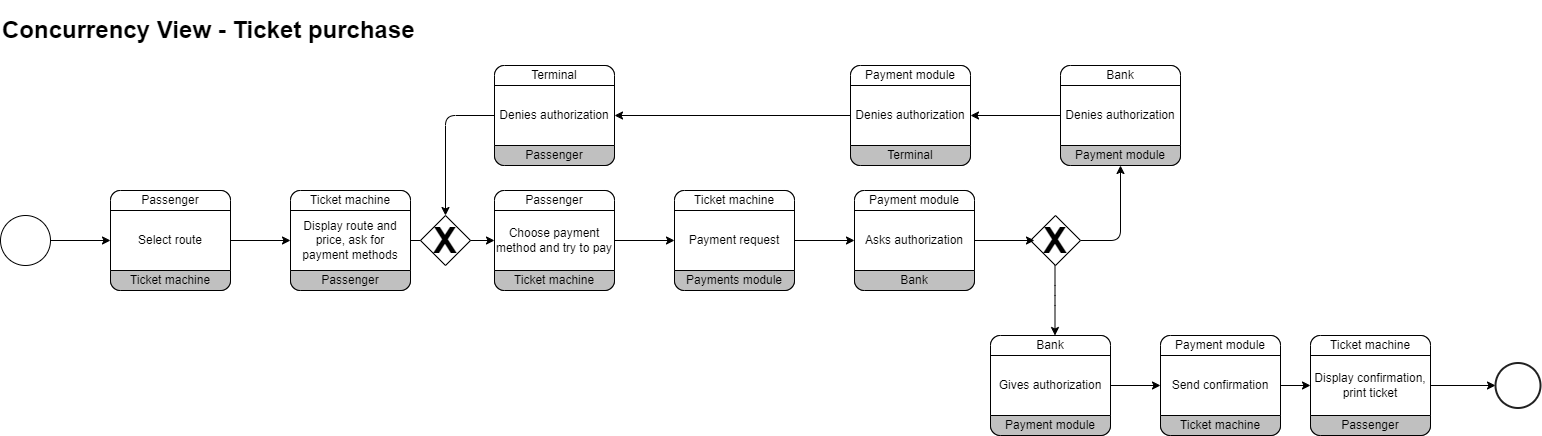
\includegraphics[width=\textwidth]{drawings/views_final_version/concurrency_view_1.png}
    \caption{Concurrency view related to ticket purchase.}
    \label{fig:concurrency_view_1}
\end{figure}

\subsection*{Description}
In the TRIP SYSTEM, the Passenger starts the process at the Ticket Machine, choosing a route and payment method. The Terminal takes over to process the payment, and the Payment Module communicates with the Bank for payment approval. If the Bank approves, the Payment Module signals the Ticket Machine to confirm the transaction and print the ticket. If the Bank denies the payment, the process is stopped, and the Passenger is notified.

\begin{table}[H]
    \centering
    \caption{Glossary for the Payment and Ticketing Process.}
    \label{tab:payment_ticketing_glossary}
    \begin{tabularx}{\textwidth}{@{}lX@{}} % Use 'X' for auto-adjusting width
    \toprule
    \textbf{Element} & \textbf{Description} \\
    \midrule
    Passenger & The customer who initiates the process by selecting a route and choosing a payment method to pay for a ticket. \\
    Ticket Machine & The interface through which the passenger selects a route, displays the route and price, and chooses a payment method. \\
    Terminal & The point of service where the passenger's payment authorization is processed. \\
    Payment Module & The system component that interacts with the bank to request payment authorization for the transaction. \\
    Bank & The financial institution that either authorizes or denies the payment transaction. \\
    \bottomrule
    \end{tabularx}
\end{table}

\begin{figure}[H]
    \centering
    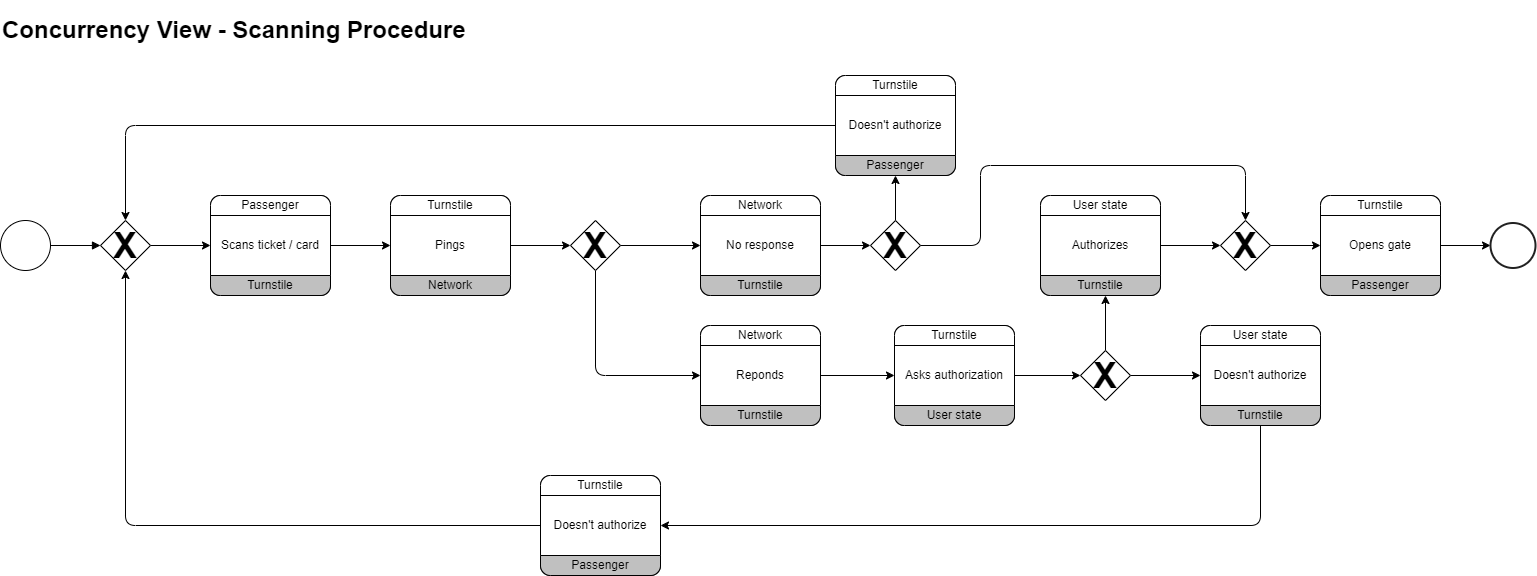
\includegraphics[width=\textwidth]{drawings/views_final_version/concurrency_view_2.png}
    \caption{Concurrency view related to the scanning procedure.}
    \label{fig:concurrency_view_2}
\end{figure}

\subsection*{Description}
The diagram depicts a turnstile access procedure with conditional paths based on network availability and user authorization. When a Passenger scans their ticket or card at the Turnstile, two scenarios can unfold:

\begin{enumerate}
    \item If the Turnstile is unable to connect to the Network (no response), it defaults to a local decision. In this case, the turnstile can still potentially authorize the passenger to proceed based on offline data or preconfigured rules.
    \item If the Turnstile connects to the Network (network responds), it then requests authorization from the User State. The User State, after evaluating the request, either grants or denies authorization:
    \begin{itemize}
        \item If the User State authorizes the request, the Turnstile receives a signal to open the gate, allowing the Passenger to pass.
        \item If the User State denies the request, the Turnstile will not open, and the Passenger is not allowed to proceed.
    \end{itemize}
\end{enumerate}

This process ensures that the system can function and provide decisions autonomously, even in the absence of network connectivity, enhancing reliability and user experience.

\begin{table}[H]
    \centering
    \caption{Glossary for Turnstile Interaction Process.}
    \label{tab:turnstile_interaction_glossary}
    \begin{tabularx}{\textwidth}{@{}lX@{}} % Use 'X' for auto-adjusting width
    \toprule
    \textbf{Component} & \textbf{Description} \\
    \midrule
    Passenger & An individual who is attempting to gain entry through the turnstile by scanning a ticket or card. \\
    Turnstile & A physical barrier at an entry point that controls access, typically based on ticket or card validation. \\
    Network & The communication system that the turnstile interfaces with to verify access rights. \\
    User State & A system component that maintains the current state of a user's access rights, determining whether entry is authorized. \\
    \bottomrule
    \end{tabularx}
\end{table}

\begin{figure}[H]
    \centering
    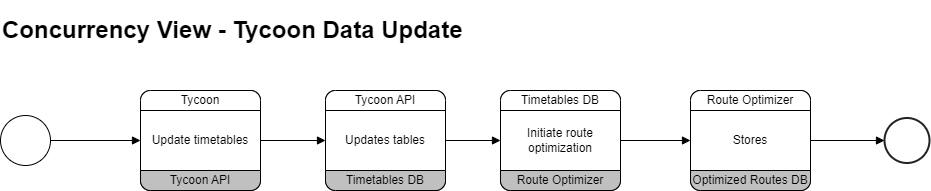
\includegraphics[width=\textwidth]{drawings/views_final_version/concurrency_view_3.png}
    \caption{Concurrency view related to tycoons data updates.}
    \label{fig:concurrency_view_3}
\end{figure}

\subsection*{Description}
This process outlines how timetable updates and route optimization are handled in the system. It begins with the Tycoon, an administrative role, who updates timetables through the Tycoon API. These updates are then applied to the Timetables DB. Following this update, the Route Optimizer initiates the optimization process, which takes the updated timetable data to determine the most efficient routes. These optimized routes are then stored in the Optimized Routes DB, completing the cycle of updating and optimizing the route information available to the system and its users.

\begin{table}[H]
    \centering
    \caption{Glossary for Route Optimization Process.}
    \label{tab:route_optimization_glossary}
    \begin{tabularx}{\textwidth}{@{}lX@{}} % Use 'X' for auto-adjusting width
    \toprule
    \textbf{Component} & \textbf{Description} \\
    \midrule
    Tycoon & Represents the train companies or transport entities responsible for managing train schedules and routes. \\
    Tycoon API & The application programming interface that allows the tycoons to update and access timetable information. \\
    Timetables DB & The database where train schedules, routes, and associated data are stored and updated. \\
    Route Optimizer & The system component that calculates the most efficient routes, likely using algorithms to process timetable data. \\
    Optimized Routes DB & A specialized database that stores the results of the route optimization process. \\
    \bottomrule
    \end{tabularx}
\end{table}

\subsection{Analysis on Perspectives}
\begin{table}[h!]
    \centering
    \resizebox{\textwidth}{!}{%
    \begin{tabular}{|l|c|c|c|c|c|c|c|c|c|}
      \hline
      & Usability & Performance & Security & Modifiability & Cost Efficiency & Availability & Safety & Integrability & Maintainability \\
      \hline
      Concurrency View & 
       & % Usability
      \cellcolor{gray!30}X & % Performance (2nd priority)
       & % Security
       & % Modifiability
       & % Cost Efficiency
      \cellcolor{gray!90}X & % Availability (1st priority)
      \cellcolor{gray!60}X & % Safety
       & % Integrability
       \\ % Maintainability
      \hline
    \end{tabular}
    }
    \caption{Concurrency View Prioritized Quality Attributes}
    \label{tab:concurrency_view}
\end{table}

\subsubsection{Scenarios}
% Scenario: Ensuring Service Availability During Network Outages
\newcommand{\scenarioOneConcurrency}{
\begin{table}[H]
    \centering
    \begin{tabularx}{\textwidth}{@{} lX @{}}
    \toprule
    \textbf{Aspect} & \textbf{Details} \\
    \midrule
    Source & Network outage impacting the TrIP system's connectivity. \\
    Stimulus & A passenger attempts to validate their ticket at a turnstile during the outage. \\
    Artifact & Hybrid approach of delayed processing and local caching implemented in the TrIP system. \\
    Response & The turnstile, equipped with local caching, validates the passenger's ticket against stored data, allowing entry. Transaction details are queued for delayed processing once network connectivity resumes, ensuring no service disruption. \\
    Measure & Passenger service continuity is maintained with 99.9\% uptime, and ticket validations during outages show no significant delay, ensuring high system availability. \\
    \bottomrule
    \end{tabularx}
    \caption{Scenario for Availability - Network Outage Handling}
    \label{table:availability_network_outage}
\end{table}
}
% Scenario: Maintaining Safety through Authorized Access

\newcommand{\scenarioTwoConcurrency}{
\begin{table}[H]
    \centering
    \begin{tabularx}{\textwidth}{@{} lX @{}}
    \toprule
    \textbf{Aspect} & \textbf{Details} \\
    \midrule
    Source & TrIP system's safety protocols for access control. \\
    Stimulus & An individual attempts to access the transit system without a valid ticket or permission. \\
    Artifact & Turnstile with integrated validation system that checks for valid tickets. \\
    Response & The turnstile denies entry to the individual without a valid ticket, preventing unauthorized access and maintaining the safety and security of the transit environment. \\
    Measure & Zero reported incidents of unauthorized access, ensuring the safety of the transit system and its users. \\
    \bottomrule
    \end{tabularx}
    \caption{Scenario for Safety - Authorized Access Enforcement}
    \label{table:safety_authorized_access}
\end{table}
}

% Scenario: Optimizing Performance with Pre-stored Routes
\newcommand{\scenarioThreeConcurrency}{
\begin{table}[H]
    \centering
    \begin{tabularx}{\textwidth}{@{} lX @{}}
    \toprule
    \textbf{Aspect} & \textbf{Details} \\
    \midrule
    Source & Passenger requests the best route options via the TrIP system during peak hours. \\
    Stimulus & High demand for route information causes potential strain on the system. \\
    Artifact & Optimized Routes Database that stores frequently requested route data. \\
    Response & The TrIP system quickly retrieves optimized route options from the pre-stored data, providing the passenger with fast and efficient service without needing to compute the routes in real-time. \\
    Measure & The response time for route information requests during peak periods remains under 2 seconds, enhancing the overall performance of the system. \\
    \bottomrule
    \end{tabularx}
    \caption{Scenario for Performance - Efficient Route Retrieval}
    \label{table:performance_route_optimization}
\end{table}
}

The Concurrency Viewpoint is central to the TRiP system's architecture, focusing on ensuring that user interactions with the system occur smoothly and without delay, even when multiple operations are executed simultaneously. This viewpoint addresses the system's capacity to manage concurrent actions effectively, with a particular emphasis on maintaining performance, safety, and availability. \\

\noindent\textbf{Ticket Purchasing Process:} \\
The sequence begins with the passenger selecting a route and payment method via the Ticket Machine. This process is crucial for performance, as it demands a fast and seamless operation to prevent queues and delays. Once the payment method is chosen, the Terminal communicates with the Payment Module to process the transaction. The Payment Module's role here is two-fold: to ensure the safety of the transaction by validating payment with the bank and to maintain the system's performance by providing quick feedback to the Terminal. If the bank authorizes the payment, the Payment Module prompts the Ticket Machine to dispense a ticket, showcasing the system's availability to complete transactions without delay. In case of a denial, the passenger is promptly informed, allowing them to take alternative actions, which is vital for maintaining system usability and ensuring the passenger's experience remains positive. \\

\noindent \textbf{Turnstile Access Control:} \\
The second aspect of concurrency comes into play at the turnstiles, where passengers scan their tickets or cards to gain access to the transport services. In this operation, the system's availability and safety are the primary concerns. The Turnstile must quickly authorize entry to avoid creating bottlenecks, which it does by pinging the Network to retrieve the User State information. If the Network is unresponsive, the Turnstile uses locally cached data to make an authorization decision, ensuring continuous operation and thus maintaining high availability. When the Network responds, the User State determines access permission. This dual approach ensures that access control is robust against network issues, preserving the integrity of operations and passenger safety by preventing unauthorized access. \\

\noindent \textbf{Route Optimization Updates:} \\
Finally, the system’s capacity to update and optimize routes through the Tycoon API and Route Optimizer reflects its modifiability and performance attributes. Tycoons can update timetables, which are then processed to optimize routes, and these optimizations are stored in the Optimized Routes DB for quick retrieval. This ensures that passengers receive up-to-date and efficient routing information, which is especially important during peak traffic conditions. \\

By detailing these processes, the concurrency viewpoint showcases the TrIP system's capability to maintain a high level of service and security across its operations, aligning with the defined quality attributes of performance, safety, and availability.

\section{Deployment Viewpoint}

\begin{figure}[H]
    \centering
    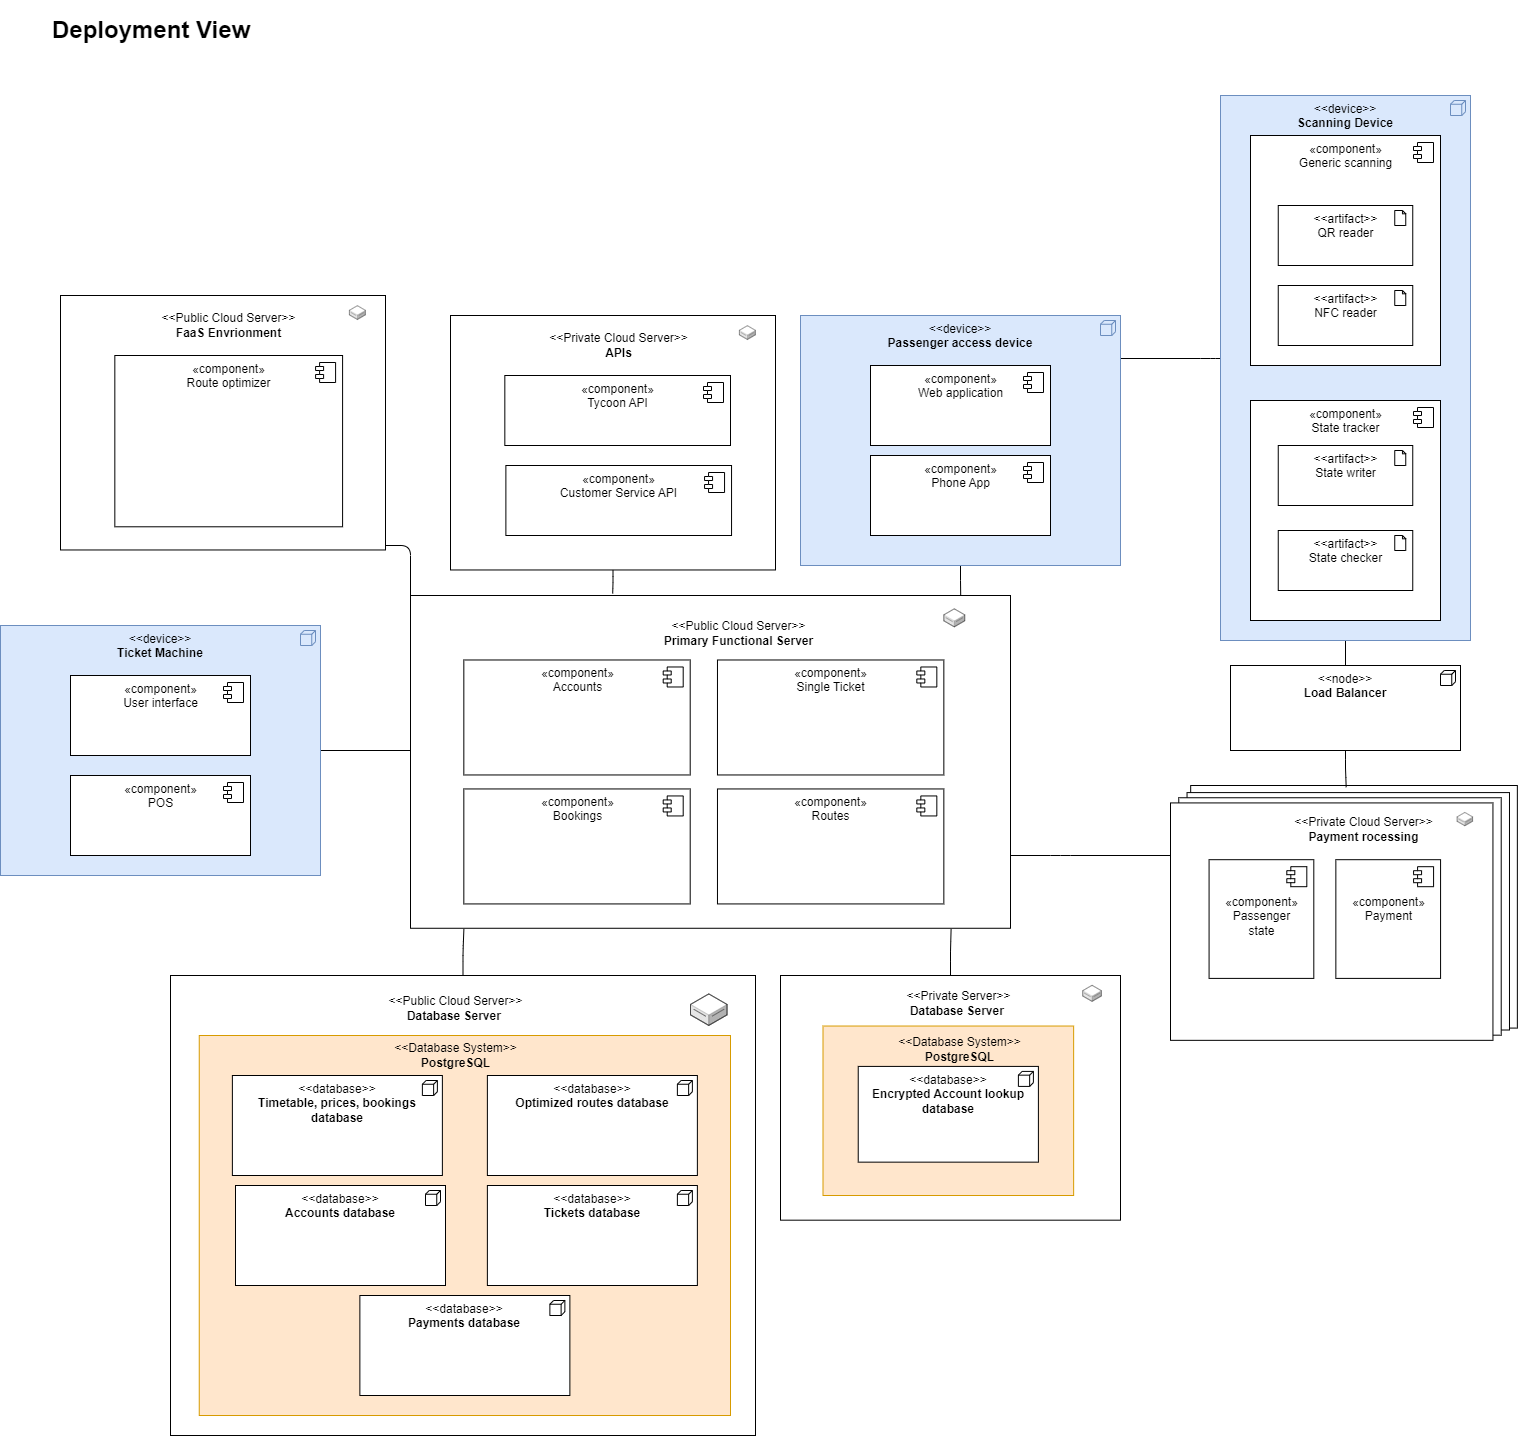
\includegraphics[width=\textwidth]{drawings/views_final_version/deployment_view.png}
    \caption{Deployment view related to the scanning procedure.}
    \label{fig:deployment_view_scanning}
\end{figure}

\subsection*{Description}
The deployment view diagram illustrates the TrIP system's architecture, showing components distributed across public and private cloud servers. Public cloud servers house the FaaS Environment for route optimization, a Terminal with Customer Service API, and the Primary Functional Server hosting Accounts, Single Ticket, Bookings, and Routes components. Devices for passenger access, such as web and phone apps, interface with scanning devices like QR and NFC readers, managed by state trackers and checkers.

The ticket machine interfaces include User Interface and POS components. Database servers in the public cloud manage the PostgreSQL databases for Timetables, Prices, Bookings, Optimized Routes, Accounts, Tickets, and Payments. The private cloud server secures the Encrypted Account Lookup database. A Load Balancer ensures efficient traffic management.

Payment processing, crucial for managing Passenger State and payments, is securely handled in the private cloud, emphasizing the system's focus on security and reliable transaction handling. 


\begin{table}[H]
    \centering
    \caption{Glossary for the Deployment View of the TrIP SYSTEM.}
    \label{tab:deployment_view_glossary}
    \begin{tabularx}{\textwidth}{@{}lXX@{}} % Corrected to have three columns
    \toprule
    \textbf{Component} & \textbf{Description} & \textbf{Hosted On} \\
    \midrule
    FaaS Environment & Provides a platform for executing backend functions in a serverless architecture, such as route optimization. & Public Cloud Servers \\
    Tycoon API & Interfaces allowing tycoons' software and systems to communicate with the TrIP system. & Private Cloud Servers \\
    Customer Service API & Facilitates customer service operations by providing data access and manipulation capabilities. & Private Cloud Servers \\
    Passenger Access Device & Equipment that passengers interact with to access the system, like ticket validation and purchases. & Terminal, App, Website \\
    Ticket Machine & Physical machines where passengers can purchase tickets and manage their bookings. & Station Locations \\
    Scanning Device & Tools used for reading ticket information, necessary for entry validation and passenger tracking. & Entry/Exit Gates \\
    QR Reader & Specialized scanners that interpret QR codes on tickets for entry validation or information retrieval. & Scanning Devices \\
    NFC Reader & Contactless devices that read NFC tags for authentication and ticket validation. & Passenger Access Devices \\
    Timetable, Prices, Bookings Database & Stores all relevant data for scheduling, pricing, and passenger bookings. & Public Cloud Servers \\
    Optimized Routes Database & Contains data on the most efficient routes calculated by the optimization algorithms. & Public Cloud Servers \\
    Accounts Database & Manages passenger account information, including subscription details and personal data. & Public Cloud Servers \\
    Tickets Database & Holds data related to ticket sales, validations, and historical transactions. & Public Cloud Servers \\
    Payments Database & Processes and records all payment transactions within the system. & Public Cloud Servers \\
    Encrypted Account Lookup Database & A secure database that stores sensitive account information, accessible only through authorized queries. & Private Cloud Servers \\
    \bottomrule
    \end{tabularx}
\end{table}

\subsection{Analysis on Perspectives}
\begin{table}[h!]
    \centering
    \resizebox{\textwidth}{!}{%
    \begin{tabular}{|l|c|c|c|c|c|c|c|c|c|}
      \hline
      & Usability & Performance & Security & Modifiability & Cost Efficiency & Availability & Safety & Integrability & Maintainability \\
      \hline
      Deployment View & 
       & % Usability
      \cellcolor{gray!90}X & % Performance (1st priority)
      \cellcolor{gray!60}X & % Security (3rd priority)
       & % Modifiability
       & % Cost Efficiency
       & % Availability (2nd priority)
       & % Safety
       & % Integrability
       \\ % Maintainability
      \hline
    \end{tabular}
    }
    \caption{Deployment View Prioritized Quality Attributes}
    \label{tab:deployment_view}
\end{table}

\subsubsection{Scenarios}
% Scenario: Upgrading Cloud Infrastructure for High Demand
\begin{table}[H]
    \centering
    \begin{tabularx}{\textwidth}{@{} lX @{}}
    \toprule
    \textbf{Aspect} & \textbf{Details} \\
    \midrule
    Source & TrIP system experiencing a surge in demand due to a new university opening at a station. \\
    Stimulus & Passenger numbers have more than quadrupled, causing performance delays during rush hours. \\
    Artifact & The deployment of the TrIP system across public cloud servers and private cloud servers. \\
    Response & The system's cloud infrastructure is updated to leverage elastic scaling capabilities. Load balancers distribute the increased traffic efficiently, and additional computing resources are allocated to handle the high load, particularly for route optimization and payment processing components. \\
    Measure & Post-update, the TrIP system handles a fourfold increase in user load with response times reduced by 70\%, ensuring that all passengers complete their transactions and receive route information within 2 seconds, even during peak rush hours. \\
    \bottomrule
    \end{tabularx}
    \caption{Scenario for Performance - Cloud Infrastructure Scaling}
    \label{table:performance_scaling}
\end{table}

% Scenario: Reinforcement of Data Security and Privacy Protocols
\begin{table}[H]
    \centering
    \begin{tabularx}{\textwidth}{@{} lX @{}}
    \toprule
    \textbf{Aspect} & \textbf{Details} \\
    \midrule
    Source & TrIP system architecture analysis in response to a competitor's security breach. \\
    Stimulus & The need to verify and bolster the security measures in place to protect passenger data. \\
    Artifact & Deployment architecture of the TrIP system with a focus on data servers and encryption protocols. \\
    Response & The system utilizes advanced encryption for data at rest and in transit within private cloud servers. Access controls are strictly enforced, ensuring only authenticated and authorized components interact with sensitive data. Periodic security audits and real-time intrusion detection systems are in place to monitor and immediately respond to any unauthorized access attempts. \\
    Measure & Security tests confirm no data leakage, and the system's compliance with the latest privacy regulations is validated by a third-party security firm, ensuring that the board and tycoons have verifiable assurance of the system's security measures. \\
    \bottomrule
    \end{tabularx}
    \caption{Scenario for Security - Privacy and Data Protection}
    \label{table:security_privacy}
\end{table}


In the Deployment Viewpoint, the TRiP system's architecture is strategically distributed across a combination of cloud-based and localized servers to optimize for both performance and security, critical attributes for the robustness and reliability of the system.

The TRiP system's deployment on cloud servers is engineered to enhance performance. The public cloud servers provide a scalable Fast Environment for handling dynamic user demands and instantaneous Route Optimization, ensuring that the most efficient paths are always available to the user. This optimization is further supported by Load Balancers, which are essential in managing network traffic by distributing workloads evenly, thereby preventing any server from becoming a bottleneck and ensuring a smooth user experience. 

For security, the system employs private cloud servers, where sensitive components such as the Encrypted Account Lookup Database are hosted. The encryption of this database is a crucial security measure, safeguarding personal and travel data against unauthorized access. 

Through this architecture, the TRiP system ensures the system is able handle the performance requirements from its users, while keeping the user information secure. Usage of cloud servers ensures dynamically scalable performance requirements. Keeping the state of the users, and caching optimzied routes is another architectural decision where the system is able to respond user requests fast with the scanning devices.

\section{Development Viewpoint}

\begin{figure}[H]
    \centering
    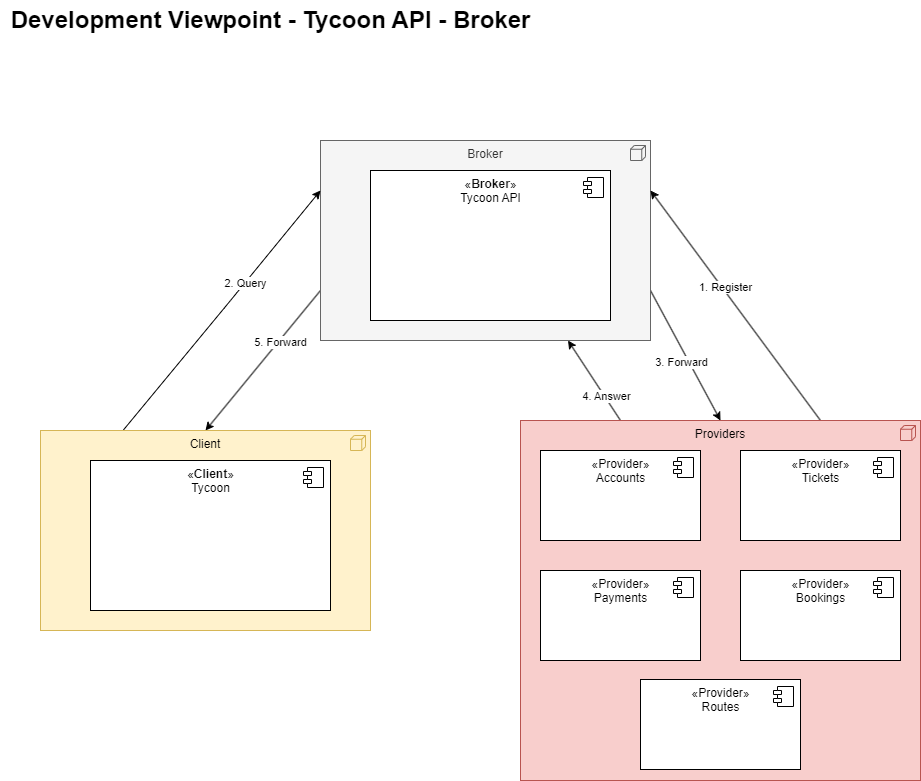
\includegraphics[width=\textwidth]{drawings/views_final_version/development_view_broker.png}
    \caption{Deployment view related broker pattern related to Tycoon API.}
    \label{fig:development_view_broker}
\end{figure}

\subsection*{Description}
The diagram portrays the broker architecture in the TrIP system, delineating the communication between clients, the broker, and providers. Tycoon clients initiate the interaction by registering with the Tycoon API broker. Queries are sent from the Tycoon to the broker, which then forwards these queries to the relevant providers. These providers include services for Accounts, Payments, Bookings, Tickets, and Routes, each playing a pivotal role in processing Tycoon requests. Upon gathering the necessary data or performing the required actions, providers send their response back to the broker. The broker, in turn, forwards this information back to the Tycoon client, completing the request-response cycle. This broker pattern facilitates a structured approach to handling requests and centralizes the communication logic, simplifying interactions across the system’s diverse components.


\begin{table}[H]
    \centering
    \caption{Glossary for the Broker in the Development View.}
    \label{tab:broker_development_glossary}
    \begin{tabular}{@{}llp{10cm}@{}}
        \toprule
    \textbf{Id} & \textbf{Name} & \textbf{Description} \\
    \midrule
    1 & Client & Represents the Tycoon requesting data or action from the broker. \\
    2 & Broker & Tycoon API that mediates between clients (Tycoon's) and various service providers (TrIP System's modules), handling requests and responses. \\
    3 & Provider & TrIP system that register with the broker to offer their services to clients. \\
    4 & Tycoon API & The application programming interface provided by the broker for communication with clients and providers. \\
    5 & Query & A request sent from the client to the broker, seeking information or action. \\
    6 & Register & The action of a provider adding their services to the broker's list of available resources. \\
    7 & Forward & The process of the broker sending requests to providers or responses back to clients. \\
    8 & Answer & The provider's response to a query that is sent back to the client via the broker. \\
    9 & Accounts & TrIP System module that manages user account information and authentication. \\
    10 & Tickets & TrIP system for issuing tickets, usually related to events or transportation. \\
    11 & Payments & The TrIP module that handles transaction processing. \\
    12 & Bookings & TrIP System module that manages reservations for services offered by the provider. \\
    13 & Routes & TrIP System module that handles route pricing. \\
    \bottomrule
    \end{tabular}
\end{table}


\begin{figure}[H]
    \centering
    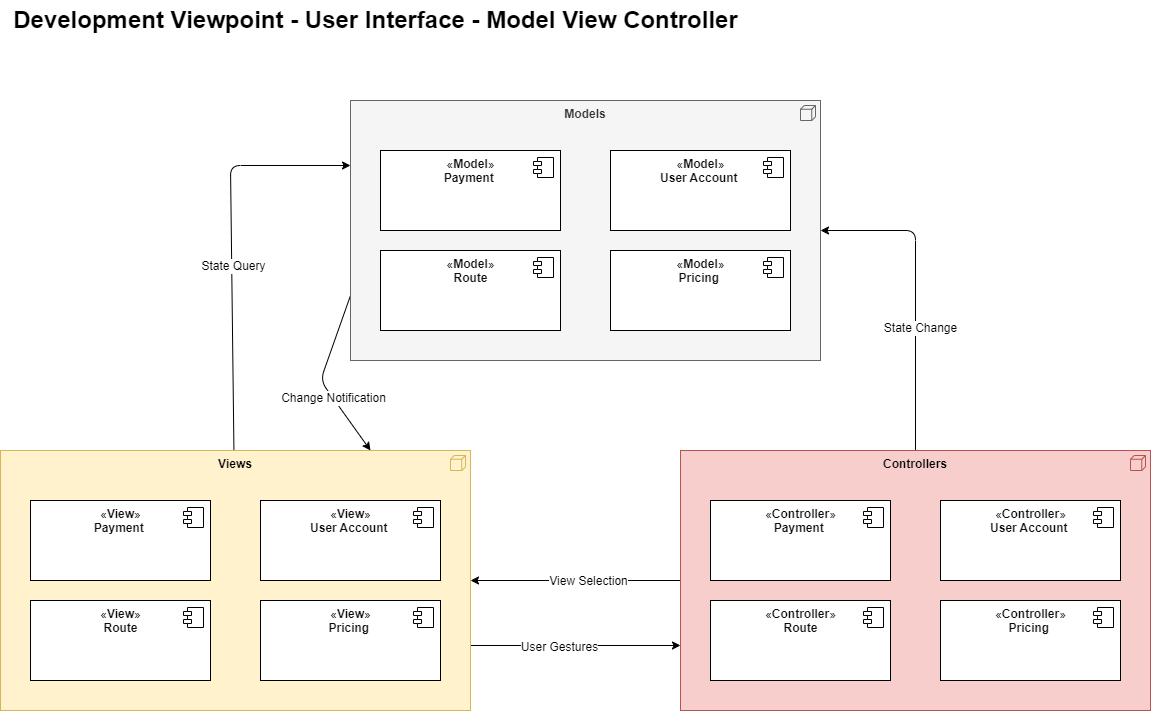
\includegraphics[width=\textwidth]{drawings/views_final_version/development_view_User_Interface.png}
    \caption{Development view model-view-controller pattern for UI}
    \label{fig:development_view_User_Interface}
\end{figure}

\subsection*{Description}
This diagram illustrates the Model-View-Controller (MVC) pattern applied within the TrIP system. It breaks down the system's user interface into Views, which are responsible for presenting data to users and include interfaces for Payment, User Account, Route, and Pricing. The Models act as the data layer with Payment, Route, User Account, and Pricing components that manage the system's state. They receive state queries and broadcast state changes to the Views. Controllers interpret user gestures, direct state changes, and mediate between the Models and Views. This separation of concerns ensures that user interactions are handled efficiently, system data is managed cohesively, and business logic is executed in a controlled manner. The MVC architecture is fundamental to the system's organization, promoting clear delineations between different functionalities and facilitating ease of maintenance and scalability.

\begin{table}[H]
    \centering
    \caption{Legend for the User Interface Components in the Development View of the TrIP System.}
    \label{tab:trip_system_ui_development_legend}
    \begin{tabular}{@{}llp{10cm}@{}}
    \toprule
    \textbf{Id} & \textbf{Name} & \textbf{Description} \\
    \midrule
    1 & Views & User interface components of the TrIP system that passengers interact with, including elements like payment, account management, and route selection screens. \\
    2 & Models & Data structures in the TrIP system that encapsulate the core business logic related to payment, user accounts, route information, and pricing. \\
    3 & Controllers & Components within the TrIP system that manage input from passengers, process requests, and produce responses by interacting with Models and updating Views. \\
    4 & Payment View/Model/Controller & Dedicated interfaces, data, and logic for processing passenger payments within the TrIP system, ensuring secure transactions. \\
    5 & User Account View/Model/Controller & Elements responsible for managing passenger profiles, including authentication and handling of personal account details in the TrIP system. \\
    6 & Route View/Model/Controller & Components that handle the presentation, data management, and operational logic of travel routes available to passengers in the TrIP system. \\
    7 & Pricing View/Model/Controller & The set of user interfaces, algorithms, and data that determine and manage fare calculations and display pricing information to passengers. \\
    8 & State Query & A request by the TrIP system to retrieve the current state, such as checking a passenger's account status or ticket validity. \\
    9 & State Change & An update within the TrIP system that alters the current state in response to passenger actions or other operational changes. \\
    10 & Change Notification & A notification mechanism that informs the TrIP system and passengers when a significant change has occurred, such as a payment confirmation or route update. \\
    11 & User Gestures & Interactions by passengers with the TrIP system, like touch or click actions, which are interpreted as commands to navigate or provide input. \\
    12 & View Selection & The process within the TrIP system for choosing the appropriate user interface view to display to passengers based on the current context or request. \\
    \bottomrule
    \end{tabular}
\end{table}

\subsection{Analysis on Perspectives}
\begin{table}[h!]
    \centering
    \resizebox{\textwidth}{!}{%
    \begin{tabular}{|l|c|c|c|c|c|c|c|c|c|}
      \hline
      & Usability & Performance & Security & Modifiability & Cost Efficiency & Availability & Safety & Integrability & Maintainability \\
      \hline
      Development View & 
      \cellcolor{gray!60}X & % Usability (2nd priority)
       & % Performance
       & % Security
       \cellcolor{gray!40}X& % Modifiability
       & % Cost Efficiency
       & % Availability
       & % Safety
       \cellcolor{gray!25}X& % Integrability
      \cellcolor{gray!90}X \\ % Maintainability (1st priority)
      \hline
    \end{tabular}
    }
    \caption{Development View Prioritized Quality Attributes}
    \label{tab:development_view}
\end{table}


\subsubsection{Scenarios}
% Scenario 1: Usability Enhancement through Standardized UIs
% Scenario: Efficient Data Retrieval for Tycoon Route Analysis and Account Information
\begin{table}[H]
    \centering
    \begin{tabularx}{\textwidth}{@{} lX @{}}
    \toprule
    \textbf{Aspect} & \textbf{Details} \\
    \midrule
    Source & Tycoon's analytical system requesting data for route pricing and passenger account details. \\
    Stimulus & The Tycoon system sends a data request to analyze route prices based on their subscription models and to gather specific account information for passengers. \\
    Artifact & Tycoon API interfacing between the Tycoon's systems and the TrIP system's databases. \\
    Response & The Tycoon API promptly routes the queries to the appropriate data providers, retrieves the requested information, and consolidates the results for the Tycoon system. \\
    Measure & Tycoon system receives comprehensive data within 3 seconds, enabling effective route and subscription analysis for passenger accounts. \\
    \bottomrule
    \end{tabularx}
    \caption{Scenario for Tycoon API Data Retrieval}
    \label{table:tycoon_api_data_retrieval}
\end{table}

% Scenario: Streamlined System Updates through MVC Pattern
\begin{table}[H]
    \centering
    \begin{tabularx}{\textwidth}{@{} lX @{}}
    \toprule
    \textbf{Aspect} & \textbf{Details} \\
    \midrule
    Source & TrIP system development team. \\
    Stimulus & The need to update the route pricing algorithm without affecting the user interface. \\
    Artifact & Model-View-Controller (MVC) pattern within the TrIP system. \\
    Response & Developers update the Pricing Model with the new algorithm, which automatically propagates changes to the relevant Views without requiring additional adjustments. \\
    Measure & The system update is deployed with zero downtime, and subsequent feature updates require 40\% less time due to decoupled architecture. \\
    \bottomrule
    \end{tabularx}
    \caption{Scenario for Maintainability - MVC Pattern}
    \label{table:mvc_maintainability}
\end{table}

% Scenario: Enhanced User Experience with MVC-Driven UI
\begin{table}[H]
    \centering
    \begin{tabularx}{\textwidth}{@{} lX @{}}
    \toprule
    \textbf{Aspect} & \textbf{Details} \\
    \midrule
    Source & Passenger using the TrIP system to manage travel. \\
    Stimulus & The passenger updates their travel preferences in the User Account View. \\
    Artifact & MVC pattern facilitating the User Account management. \\
    Response & The Controller processes the passenger's input, updates the User Account Model, and the View dynamically reflects the changes, providing immediate visual confirmation to the passenger. \\
    Measure & Passengers express a 90\% satisfaction rate with the ease of updating preferences, and the error rate in preference updates decreases by 50\%. \\
    \bottomrule
    \end{tabularx}
    \caption{Scenario for Usability - MVC-Driven UI}
    \label{table:mvc_usability}
\end{table}

The Development Viewpoint focuses on the structural aspects that underpin the TrIP system's architecture, highlighting the modular approach in system design to enhance usability and maintainability. \\

\noindent \textbf{MVC Pattern:} \\
The adoption of the Model-View-Controller (MVC) pattern substantially improves the system's maintainability by segregating the user interface elements (Views) from the business logic (Models) and user input processing (Controllers). This separation of concerns allows developers to update or modify one aspect of the system — such as adding new features to the user interface — without the need to alter the underlying business logic or control flow. For passengers, this results in a more comprehensive interface with a variety of options and features, enhancing the overall usability of the system. The MVC pattern ensures that as passenger needs evolve, new Views can be added swiftly, making the system both adaptable and future-proof. \\

\noindent \textbf{Broker Architecture:} \\
In parallel, the broker architecture employed within the Tycoon API streamlines the interaction process between the Tycoons and the TrIP system. It serves as a centralized point for processing queries and handling communications, thus simplifying the complexity of these interactions. For the Tycoons, this architecture means usability is significantly enhanced, allowing them to communicate through a unified interface with the Tycoon API, which abstracts the intricate workings of the TrIP system's service modules. This consolidation of communication logic not only benefits the Tycoons but also reduces the overhead for the TrIP system in managing multiple communication protocols. \\

These architectural decisions, reflected in the Development Viewpoint, are key to the TrIP system's ability to offer an efficient, secure, and user-friendly platform that can grow and adapt in line with technological advancements and user expectations.


\appendix

\section{User Stories}

\subsection{Prioritized User Stories}
The prioritization of selected user stories focuses on core objectives such as enhancing passenger experience, ensuring security, promoting operational efficiency, and facilitating seamless integration:

\begin{itemize}
    \item \textbf{User Stories 1 and 16} simplify the payment process, enhancing usability and convenience across multiple networks.
    \item \textbf{User Story 18} secures personal and financial data, aligning with trust-building and regulatory compliance.
    \item \textbf{User Story 29} underlines operational cost-efficiency, vital for the system's sustainability.
    \item \textbf{User Story 23} ensures smooth integration with existing railroad infrastructure, key to operational continuity and adoption.
    \item \textbf{User Stories 4 and 7} use technology to improve accessibility and the user experience, making the system inclusive.
    \item \textbf{User Stories 26 and 27} highlight adaptability in maintenance and scheduling, crucial for service quality and minimizing passenger disruption.
\end{itemize}

Prioritizing these stories ensures the system meets crucial user needs and operational objectives, setting a foundation for success and growth.

\subsection{Passengers}
\begin{itemize}
    \item \userStoryOne
    \item \userStoryTwo
    \item \userStoryThree
    \item \userStoryThirtySeven
    \item \userStoryThirtyNine
\end{itemize}

\subsection{Tech-savvy Passengers}
\begin{itemize}
    \item \userStoryFour
    \item \userStoryFive
\end{itemize}

\subsection{Accessibility Advocates}
\begin{itemize}
    \item \userStorySix
    \item \userStorySeven
    \item \userStoryEight
    \item \userStoryNine
    \item \userStoryTen
\end{itemize}

\subsection{Passengers with Special Considerations}
\begin{itemize}
    \item \userStoryEleven
    \item \userStoryTwelve
    \item \userStoryThirteen
    \item \userStoryFourteen
    \item \userStoryFifteen
    \item \userStorySixteen
    \item \userStorySeventeen
\end{itemize}

\subsection{Government}
\begin{itemize}
    \item \userStoryEighteen
    \item \userStoryNineteen
    \item \userStoryTwenty
\end{itemize}

\subsection{Tycoons (Train Company Owners)}
\begin{itemize}
    \item \userStoryTwentyOne
    \item \userStoryTwentyTwo
    \item \userStoryTwentyThree
    \item \userStoryTwentyFour
    \item \userStoryThirtyFive
    \item \userStoryThirtyEight
    \item \userStoryForty
\end{itemize}

\subsection{Financial Analysts}
\begin{itemize}
    \item \userStoryTwentyFive
\end{itemize}

\subsection{Station Staff}
\begin{itemize}
    \item \userStoryTwentySix
\end{itemize}

\subsection{Maintenance Teams}
\begin{itemize}
    \item \userStoryTwentySeven
\end{itemize}

\subsection{Government Financial Auditors}
\begin{itemize}
    \item \userStoryTwentyEight
\end{itemize}

\subsection{TrIP Owner}
\begin{itemize}
    \item \userStoryFortyOne
    \item \userStoryTwentyNine
    \item \userStoryThirty
    \item \userStoryThirtyOne
    \item \userStoryThirtyTwo
    \item \userStoryThirtyThree
    \item \userStoryThirtyFour
\end{itemize}

\subsection{System administrator}
\begin{itemize}
    \item \userStoryThirtySix
\end{itemize}

% \begin{table}[H]
    \resizebox{\textwidth}{!}{%
    \begin{tabular}{|l|c|c|c|c|c|c|c|c|c|c|c|}
    \hline
    \textbf{User Story} & \textbf{Usability} & \textbf{Performance} & \textbf{Security} & \textbf{Modifiability} & \textbf{Deployability} & \textbf{Energy Efficiency} & \textbf{Availability} & \textbf{Safety} & \textbf{Integrability} & \textbf{Testability} & \textbf{Accessibility} \\
    \hline
    1. Frequent traveler monthly pass & + &  &  &  &  &  &  &  &  &  &  \\
    \hline
    2. Check travel card balance & + &  &  &  &  &  &  &  &  &  &  \\
    \hline
    3. Subscription notifications & + &  &  &  &  &  &  &  &  &  &  \\
    \hline
    4. Mobile app management & + &  &  &  & - &  &  &  &  &  &  \\
    \hline
    5. Carbon footprint tracking &  & - &  &  &  & + &  &  &  &  &  \\
    \hline
    6. Accessible services info & + &  &  &  &  &  &  & + &  &  &  \\
    \hline
    7. Voice-activated features & + &  &  & - & - &  &  &  &  &  & + \\
    \hline
    8. Simple interface for elders & + &  &  & + &  &  &  &  &  &  &  \\
    \hline
    9. Multilanguage options & + &  &  & - &  &  &  &  &  &  &  \\
    \hline
    10. Quick access to popular trips & + & - &  & - &  &  &  &  &  &  &  \\
    \hline
    11. Scan student card for benefits & + &  &  & - &  &  &  &  &  &  &  \\
    \hline
    12. Single transaction for subscriptions & + & - &  &  &  &  &  &  &  &  &  \\
    \hline
    13. Charge train cards at terminal & + &  &  & - &  &  &  &  &  &  &  \\
    \hline
    14. Interface for visually impaired & + &  &  &  &  &  &  &  &  &  & + \\
    \hline
    15. Block payment for blocked routes & + & - &  & - &  &  &  &  &  &  &  \\
    \hline
    16. Single ticket across all networks & + & - &  & - &  &  &  &  &  &  &  \\
    \hline
    17. Subscriptions advice for commuting & + & - &  & - &  &  &  &  &  &  &  \\
    \hline
    18. Adherence to security standards &  &  & + & - &  &  &  &  & - & - &  \\
    \hline
    19. Detailed reporting for government & + &  &  & - &  &  &  &  & - &  &  \\
    \hline
    20. Reduced fares for eligible populations & + & - &  & - &  &  &  &  &  &  &  \\
    \hline
    21. Revenue tracking for tycoons & + & - &  & - &  &  &  &  &  &  &  \\
    \hline
    22. Exclusive promotions & + &  &  & - &  &  &  &  &  &  &  \\
    \hline
    23. Payment system integration & + &  &  & - &  &  &  &  & + & - &  \\
    \hline
    24. Access to analytics &  &  &  & - &  &  &  &  & + &  &  \\
    \hline
    25. Assistance for ticket purchases & + &  &  & - &  &  &  &  &  &  &  \\
    \hline
    26. Temporary fare adjustments &  &  &  & - &  & + &  &  &  &  &  \\
    \hline
    27. Integration with maintenance tools &  &  &  & - &  & + &  &  &  &  &  \\
    \hline
    28. Audit trails and compliance &  &  &  & - &  &  &  &  &  &  &  \\
    \hline
    \end{tabular}%
    }
    \caption{User Stories and Quality Attributes}
\end{table}

\end{document}
